\documentclass{beamer}\usepackage[]{graphicx}\usepackage[]{color}
%% maxwidth is the original width if it is less than linewidth
%% otherwise use linewidth (to make sure the graphics do not exceed the margin)
\makeatletter
\def\maxwidth{ %
  \ifdim\Gin@nat@width>\linewidth
    \linewidth
  \else
    \Gin@nat@width
  \fi
}
\makeatother

\definecolor{fgcolor}{rgb}{0.345, 0.345, 0.345}
\newcommand{\hlnum}[1]{\textcolor[rgb]{0.686,0.059,0.569}{#1}}%
\newcommand{\hlstr}[1]{\textcolor[rgb]{0.192,0.494,0.8}{#1}}%
\newcommand{\hlcom}[1]{\textcolor[rgb]{0.678,0.584,0.686}{\textit{#1}}}%
\newcommand{\hlopt}[1]{\textcolor[rgb]{0,0,0}{#1}}%
\newcommand{\hlstd}[1]{\textcolor[rgb]{0.345,0.345,0.345}{#1}}%
\newcommand{\hlkwa}[1]{\textcolor[rgb]{0.161,0.373,0.58}{\textbf{#1}}}%
\newcommand{\hlkwb}[1]{\textcolor[rgb]{0.69,0.353,0.396}{#1}}%
\newcommand{\hlkwc}[1]{\textcolor[rgb]{0.333,0.667,0.333}{#1}}%
\newcommand{\hlkwd}[1]{\textcolor[rgb]{0.737,0.353,0.396}{\textbf{#1}}}%

\usepackage{framed}
\makeatletter
\newenvironment{kframe}{%
 \def\at@end@of@kframe{}%
 \ifinner\ifhmode%
  \def\at@end@of@kframe{\end{minipage}}%
  \begin{minipage}{\columnwidth}%
 \fi\fi%
 \def\FrameCommand##1{\hskip\@totalleftmargin \hskip-\fboxsep
 \colorbox{shadecolor}{##1}\hskip-\fboxsep
     % There is no \\@totalrightmargin, so:
     \hskip-\linewidth \hskip-\@totalleftmargin \hskip\columnwidth}%
 \MakeFramed {\advance\hsize-\width
   \@totalleftmargin\z@ \linewidth\hsize
   \@setminipage}}%
 {\par\unskip\endMakeFramed%
 \at@end@of@kframe}
\makeatother

\definecolor{shadecolor}{rgb}{.97, .97, .97}
\definecolor{messagecolor}{rgb}{0, 0, 0}
\definecolor{warningcolor}{rgb}{1, 0, 1}
\definecolor{errorcolor}{rgb}{1, 0, 0}
\newenvironment{knitrout}{}{} % an empty environment to be redefined in TeX

\usepackage{alltt}
\usetheme{Boadilla}
\usecolortheme{beaver}


\usepackage{graphicx}
\graphicspath{{../figures/}}
\usepackage{amsmath}
\usepackage{booktabs}

\author{Christof Angermueller}
\title{Statistics Introduction}
\date{\today}





\IfFileExists{upquote.sty}{\usepackage{upquote}}{}
\begin{document}

\begin{frame}
  \titlepage
\end{frame}

\begin{frame}
  \tableofcontents
\end{frame}



\section{Introduction}

\begin{frame}{About me}
  \begin{itemize}
    \item 2nd year PhD student EMBL-EBI
    \item Supervisor: Oliver Stegle
    \item Machine learning, Statistics, Biological data analysis
    \item @cangermueller
    \item \url{http://cangermueller.com}
  \end{itemize}
\end{frame}

\begin{frame}{Sequencing costs}
  \begin{itemize}
    \item Rapidly declining sequencing costs per genome
  \end{itemize}
  \begin{center}
    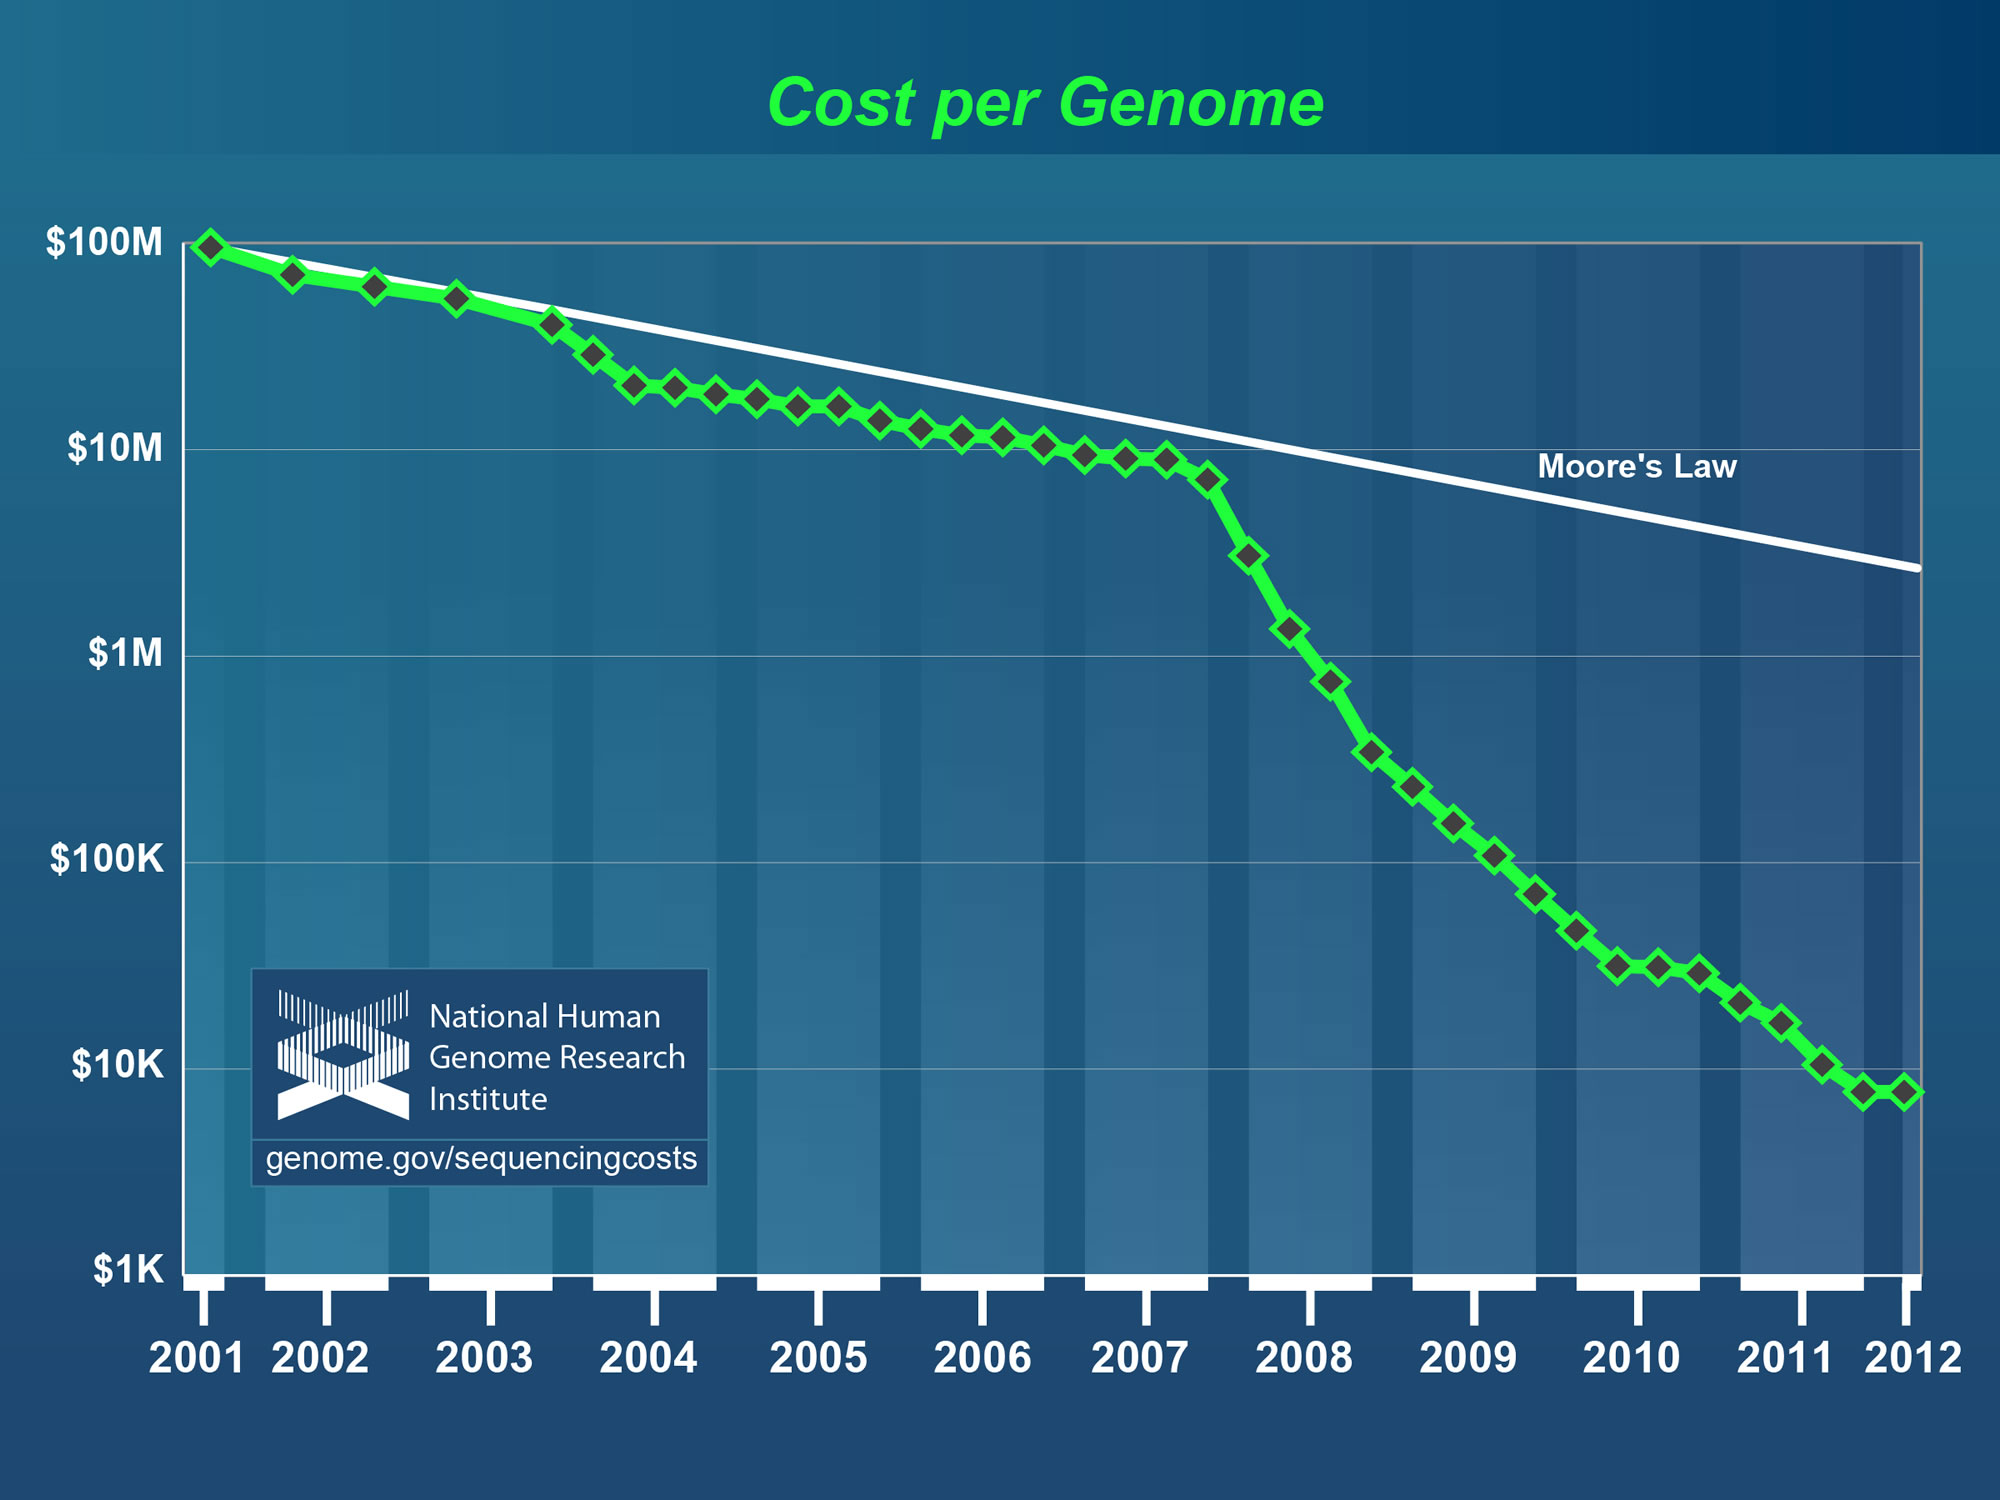
\includegraphics[width=.8\linewidth]{costs_genome.jpg}
  \end{center}
\end{frame}

\begin{frame}{Big data in biology}
  \begin{itemize}
    \item EBI stores 10 peta-bytes: 10 000 000 000 000 000 bytes
    \item 2 peta-beta bytes of genomic data
    \item {\color{red} Huge computational challenges}
    \item {\color{green} Huge biological potential}
  \end{itemize}
  \begin{center}
    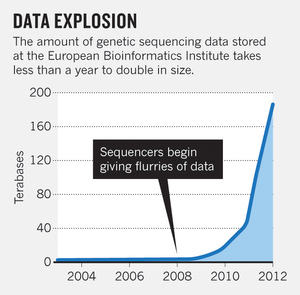
\includegraphics[width=.5\linewidth]{data_ebi.jpg}
  \end{center}
\end{frame}

\begin{frame}{Why should I care about statistics?}
  \begin{itemize}
    \item Because you can analyse your own data
    \item Because it allows you to tap the reservoir of biological data
    \item Because it increases your chance to find a job after your PhD
    \item Because it is fun!
  \end{itemize}
\end{frame}

\section{Descriptive statistics}
\begin{frame}
\tableofcontents[currentsection]
\end{frame}

\begin{frame}{Statistical inference}
  \begin{center}
    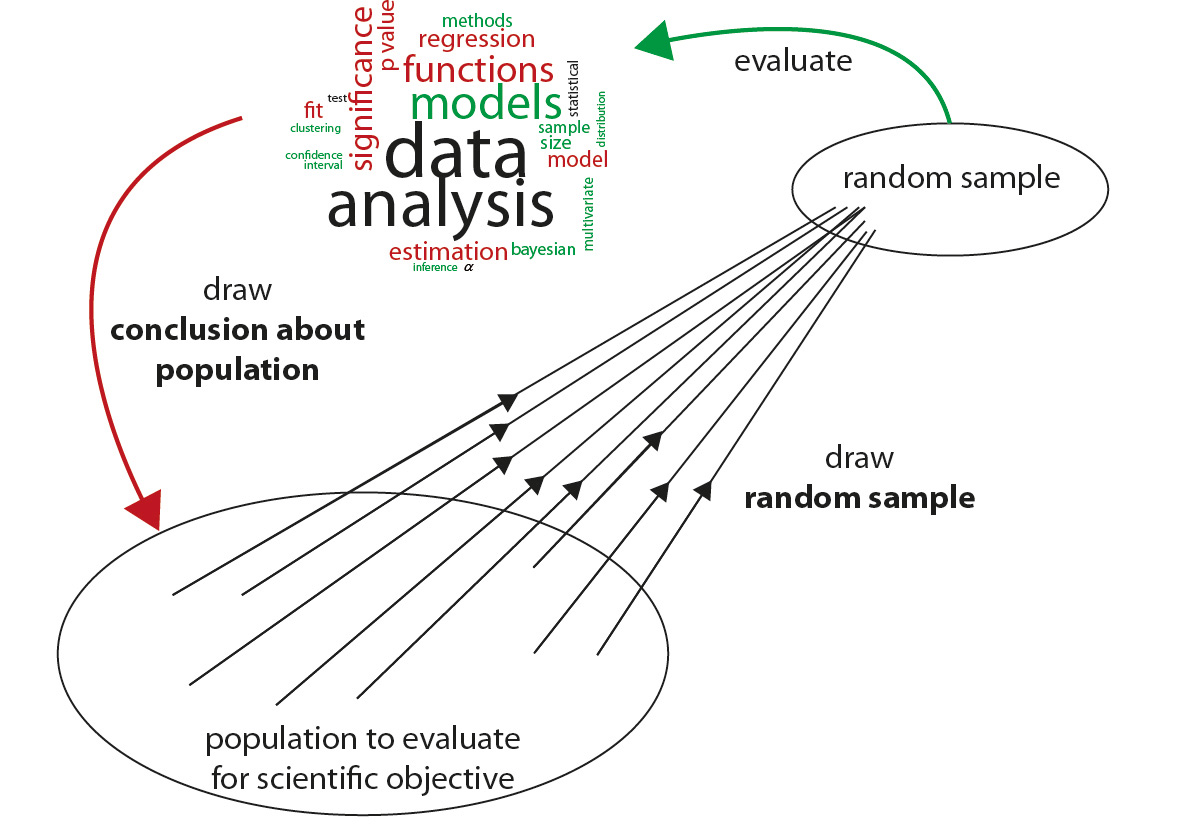
\includegraphics[width=.7\linewidth]{inference.jpg}
  \end{center}
\end{frame}

\begin{frame}{Type-1 Diabetes (T1D) data}
  \begin{itemize}
    \item $9627$ samples from human population
    \item Classified as diabetic or non-diabetic
    \item Genotyped for T1D risk genes
  \end{itemize}
  \tiny
\begin{kframe}
\begin{alltt}
\hlkwd{xtable}\hlstd{(t1d[}\hlkwd{sample}\hlstd{(}\hlkwd{nrow}\hlstd{(t1d))[}\hlnum{1}\hlopt{:}\hlnum{10}\hlstd{],])}
\end{alltt}
\end{kframe}% latex table generated in R 3.1.1 by xtable 1.7-4 package
% Fri Nov 28 08:56:51 2014
\begin{table}[ht]
\centering
\begin{tabular}{rlrlrlrrrrrr}
  \hline
 & t1d & hlacat & sex & age & european & ptpn22 & il10 & ctla4 & bach2 & erbb3 & gab3 \\ 
  \hline
8648 & yes &   1 & f & 12.32 & TRUE &   0 &   2 &   1 &   2 &   1 &   0 \\ 
  6823 & yes &   2 & m & 10.94 & TRUE &   0 &   2 &   2 &   1 &   0 &   2 \\ 
  9584 & no &   1 & m & 0.00 & TRUE &   1 &   2 &   1 &   0 &   0 &   0 \\ 
  975 & yes &   6 & f & 5.81 & TRUE &   0 &   1 &   0 &   2 &   2 &   1 \\ 
  4845 & yes &   3 & f & 10.77 & TRUE &   1 &   2 &   1 &   1 &   2 &   1 \\ 
  5323 & yes &   5 & m & 10.32 & TRUE &   1 &   0 &   1 &   1 &   2 &   0 \\ 
  3857 & yes &   3 & m & 5.95 & TRUE &   0 &   2 &   2 &   1 &   2 &   0 \\ 
  5207 & yes &   3 & m & 6.12 & TRUE &   0 &   2 &   1 &   2 &   1 &   0 \\ 
  4966 & yes &   3 & m & 7.59 & TRUE &   0 &   1 &   2 &   0 &   1 &   2 \\ 
  8647 & yes &   1 & f & 4.49 & TRUE &   0 &   2 &   0 &   2 &   1 &   1 \\ 
   \hline
\end{tabular}
\end{table}

\end{frame}

\begin{frame}{T1D variables}
  \begin{itemize}
    \item $Y$: \textbf{Output variable}, \textbf{target variable}
      \begin{itemize}
        \item T1D yes or no
      \end{itemize}
    \item $X_i$: \textbf{Input variables}, \textbf{explanatory variables}, 
      \textbf{covariates}
      \begin{itemize}
        \item Sex
        \item Age
        \item European
        \item PTPN22, IL10, CTLA4, ...
      \end{itemize}
  \end{itemize}
\end{frame}

\begin{frame}{Types of variables}
  \begin{columns}[t]
    \begin{column}{.45\linewidth}
      \begin{exampleblock}{Discrete}
        \begin{itemize}
          \item $X \in \{s_1, s_2, \dots, s_n\}$
          \item {\bf Binary} 
            \\ $\text{european} \in \{\text{TRUE}, \text{FALSE}\}$
          \item {\bf Categorical} \\ 
            $\text{sex} \in \{\text{f}, \text{m}\}$
          \item {\bf Ordinal} 
            \\ $\text{age} \in \{\text{child}, \text{adult}, \text{elder}\}$
          \item {\bf Integer} 
            \\ $\text{ptpn22} \in \{0, 1, 2\}$
        \end{itemize}
      \end{exampleblock}
    \end{column}
    \begin{column}{.45\linewidth}
      \begin{exampleblock}{Continuous}
        \begin{itemize}
          \item $X \in \mathbb{R}$
          \item $\text{age} \in [0, 0.01, \dots, \inf[$
        \end{itemize}
      \end{exampleblock}
    \end{column}
  \end{columns}
  \begin{align*}
    \text{Binary} < \text{Categorical} < \text{Ordinal} < \text{Integer} <
    \text{Continuous}
  \end{align*}
\end{frame}

\begin{frame}{Operations on variables}
  \begin{description}
    \item[Count] Binary, categorical, ordinal, integer, continuous
    \item[Median] Ordinal, integer, continuous
    \item[Median] Ordinal, integer, continuous
    \item[Mean] Integer, continuous
  \end{description}
\end{frame}

\begin{frame}[fragile]{Count}
  \begin{definition}[Count]
    \begin{itemize}
      \item How often does $x$ appear?
      \item Binary, categorical, ordinal, integer, continuous
    \end{itemize}
  \end{definition}
\begin{knitrout}\tiny
\definecolor{shadecolor}{rgb}{0.969, 0.969, 0.969}\color{fgcolor}\begin{kframe}
\begin{alltt}
\hlkwd{table}\hlstd{(t1d}\hlopt{$}\hlstd{t1d)}
\end{alltt}
\begin{verbatim}
## 
##   no  yes 
## 1766 7861
\end{verbatim}
\begin{alltt}
\hlkwd{table}\hlstd{(t1d}\hlopt{$}\hlstd{sex)}
\end{alltt}
\begin{verbatim}
## 
##    f    m 
## 4721 4906
\end{verbatim}
\end{kframe}
\end{knitrout}
\end{frame}

\begin{frame}[fragile]{Median}
  \begin{definition}[Median]
    \begin{itemize}
      \item Value in the middle
      \item Ordinal, integer, continuous
    \end{itemize}
  \end{definition}
\begin{knitrout}\tiny
\definecolor{shadecolor}{rgb}{0.969, 0.969, 0.969}\color{fgcolor}\begin{kframe}
\begin{alltt}
\hlkwd{median}\hlstd{(t1d}\hlopt{$}\hlstd{hlacat)}
\end{alltt}
\begin{verbatim}
## [1] 3
\end{verbatim}
\begin{alltt}
\hlkwd{median}\hlstd{(t1d}\hlopt{$}\hlstd{age)}
\end{alltt}
\begin{verbatim}
## [1] 7.989935
\end{verbatim}
\end{kframe}
\end{knitrout}
\end{frame}

\begin{frame}[fragile]{Quantile}
  \begin{definition}[Quantile]
    \begin{itemize}
      \item $q_p(X)$ is value $x$, s.t. $q\%$ of all $y \in Y$ are smaller than $x$
      \item $q_{0.5}(X) = \operatorname{median}(X)$
      \item Ordinal, integer, continuous
    \end{itemize}
  \end{definition}
\begin{knitrout}\tiny
\definecolor{shadecolor}{rgb}{0.969, 0.969, 0.969}\color{fgcolor}\begin{kframe}
\begin{alltt}
\hlkwd{quantile}\hlstd{(t1d}\hlopt{$}\hlstd{hlacat)}
\end{alltt}
\begin{verbatim}
##   0%  25%  50%  75% 100% 
##    1    2    3    6    6
\end{verbatim}
\begin{alltt}
\hlkwd{quantile}\hlstd{(t1d}\hlopt{$}\hlstd{age)}
\end{alltt}
\begin{verbatim}
##        0%       25%       50%       75%      100% 
##  0.000000  5.234090  7.989935 10.673839 22.137645
\end{verbatim}
\end{kframe}
\end{knitrout}
\end{frame}

\begin{frame}[fragile]{Mean}
  \begin{definition}[Mean]
    \begin{itemize}
      \item $\operatorname{mean}(X) = \frac{1}{|X|}\sum_{x \in X} x$
      \item Integer, continuous variables
    \end{itemize}
  \end{definition}
\begin{knitrout}\tiny
\definecolor{shadecolor}{rgb}{0.969, 0.969, 0.969}\color{fgcolor}\begin{kframe}
\begin{alltt}
\hlkwd{mean}\hlstd{(t1d}\hlopt{$}\hlstd{age)}
\end{alltt}
\begin{verbatim}
## [1] 7.975919
\end{verbatim}
\end{kframe}
\end{knitrout}
\end{frame}

\begin{frame}{Random variable}
  \begin{itemize}
    \item A random variable $X$ has a random outcome $x \in \mathcal{D}$
    \item $\mathcal{D}$ is the \textbf{domain} of $X$
    \item \textbf{Discrete $X$}: $\mathcal{D} \subseteq \mathbb{Z}$, e.g. $\mathbb{D}=\{0, 1, 2, \dots\}$
    \item \textbf{Continuous $X$}: $\mathcal{D} \subseteq \mathbb{R}$, e.g. $\mathbb{D}=[0.0, 0.1, 0.2, \dots[$
    \item $P(X=x)$ is the \textbf{probability} that $X$ has outcome $x$
    \item $E[X]=\sum_{x \in \mathcal{D}} P(X=x) x$ is the \textbf{expected value} of $X$
    \item $Var[X]=\sum_{x \in \mathcal{D}} P(X=x) (x - E[X])^2$ is the \textbf{variance} of $X$
    \item $Sd[X]=\sqrt{Var[X]}$ is the \textbf{standard deviation} of $X$
  \end{itemize}
\end{frame}

\begin{frame}{Discrete Random Variable}
  \begin{itemize}
    \item $f(x) = P(X=x)$ is the \textbf{Probability Mass Function (PMF)} of $X$
    \item $F(X) = P(X\le x)$ is the \textbf{Cumulative Distribution Function (CDF)} of $X$
  \end{itemize}
  \begin{exampleblock}{Examples}
    \begin{itemize}
      \item $\operatorname{Bernoulli}(p)$: $\mathcal{D} = \{0, 1\}$
      \item $\operatorname{Binomial}(n, p)$: $\mathcal{D} = \{0, 1, \dots, n\}$
      \item $\operatorname{Poisson}(\lambda)$: $\mathcal{D} = \{0, 1, \dots, +\inf\}$
    \end{itemize}
  \end{exampleblock}
\end{frame}

\begin{frame}[fragile]{Bernoulli distribution}
  \begin{itemize}
    \item The gender $X$ with $\mathcal{D}=\{f, m\}$ can be modelled as
      Bernoulli distributed:
  \end{itemize}
  \begin{columns}
    \begin{column}{.5\linewidth}
      \begin{align*}
        X \sim \operatorname{Bernoulli}(p)
      \end{align*}
      \begin{align*}
        E[X] = p
      \end{align*}
      \begin{align*}
        Var[X] = p(1-p)
      \end{align*}
    \end{column}
    \begin{column}{0.5\linewidth}
\begin{knitrout}\tiny
\definecolor{shadecolor}{rgb}{0.969, 0.969, 0.969}\color{fgcolor}\begin{kframe}
\begin{alltt}
\hlstd{p} \hlkwb{<-} \hlnum{0.65}
\hlstd{exp} \hlkwb{<-} \hlstd{p}
\hlstd{samples} \hlkwb{<-} \hlkwd{rbinom}\hlstd{(}\hlnum{100}\hlstd{,} \hlnum{1}\hlstd{, p)}
\hlkwd{hist}\hlstd{(samples,} \hlkwc{col}\hlstd{=}\hlstr{'lightblue'}\hlstd{,} \hlkwc{main}\hlstd{=}\hlstr{''}\hlstd{,} \hlkwc{xlab}\hlstd{=}\hlstr{''}\hlstd{)}
\hlkwd{abline}\hlstd{(}\hlkwc{v}\hlstd{=exp,} \hlkwc{col}\hlstd{=}\hlstr{'red'}\hlstd{,} \hlkwc{lwd}\hlstd{=}\hlnum{2}\hlstd{)}
\end{alltt}
\end{kframe}

{\centering \includegraphics[width=\linewidth]{figure/hist_bernoulli-1} 

}



\end{knitrout}
    \end{column}
  \end{columns}
\end{frame}

\begin{frame}[fragile]{Bernoulli distribution}
  \begin{itemize}
    \item What is the rate $p$ of females of T1D samples?
    \item The \textbf{maximum likelihood} estimator $\hat{p}$ of $p$ is:
      \begin{align*}
        \hat{p}=\frac{1}{n}\sum_i x_i
      \end{align*}
\begin{knitrout}\tiny
\definecolor{shadecolor}{rgb}{0.969, 0.969, 0.969}\color{fgcolor}\begin{kframe}
\begin{alltt}
\hlstd{p} \hlkwb{<-} \hlkwd{sum}\hlstd{(t1d}\hlopt{$}\hlstd{sex} \hlopt{==} \hlstr{'f'}\hlstd{)} \hlopt{/} \hlkwd{nrow}\hlstd{(t1d)}
\hlstd{p}
\end{alltt}
\begin{verbatim}
## [1] 0.4903916
\end{verbatim}
\end{kframe}
\end{knitrout}
  \end{itemize}
\end{frame}

\begin{frame}[fragile]{Binomial distribution}
  \begin{itemize}
    \item The number of females $Y$ in a new cohort of $n=50$ people is
      binomial distributed:
      \begin{align*}
        Y \sim \operatorname{Binomial}(n, p)
      \end{align*}
    \item Assume that $p=\hat{p}=0.4903916$ is the same as before ...
  \end{itemize}
\end{frame}

\begin{frame}[fragile]{Binomial distribution}
  \begin{itemize}
    \item then the probability $f(y)$ to observe $k$ females is:
  \end{itemize}
\begin{knitrout}\tiny
\definecolor{shadecolor}{rgb}{0.969, 0.969, 0.969}\color{fgcolor}\begin{kframe}
\begin{alltt}
\hlstd{n} \hlkwb{<-} \hlnum{50}
\hlstd{y} \hlkwb{<-} \hlkwd{seq}\hlstd{(}\hlnum{0}\hlstd{, n)}
\hlstd{f_y} \hlkwb{<-} \hlkwd{dbinom}\hlstd{(y, n, p)}
\hlstd{d} \hlkwb{<-} \hlkwd{data.frame}\hlstd{(}\hlkwc{x}\hlstd{=y,} \hlkwc{y}\hlstd{=f_y)}
\hlkwd{ggplot}\hlstd{(d,} \hlkwd{aes}\hlstd{(}\hlkwc{x}\hlstd{=x,} \hlkwc{y}\hlstd{=y))} \hlopt{+} \hlkwd{geom_point}\hlstd{(}\hlkwc{color}\hlstd{=}\hlstr{'blue'}\hlstd{,} \hlkwc{size}\hlstd{=}\hlnum{3}\hlstd{)} \hlopt{+} \hlkwd{xlab}\hlstd{(}\hlstr{'y'}\hlstd{)} \hlopt{+} \hlkwd{ylab}\hlstd{(}\hlstr{'f(y)'}\hlstd{)}
\end{alltt}
\end{kframe}

{\centering \includegraphics[width=.5\linewidth]{figure/fig_bin_pdf-1} 

}



\end{knitrout}
\end{frame}

\begin{frame}[fragile]{Binomial distribution}
  \begin{itemize}
    \item and the probability $F(Y)$ to observe up to $k$ females:
  \end{itemize}
\begin{knitrout}\tiny
\definecolor{shadecolor}{rgb}{0.969, 0.969, 0.969}\color{fgcolor}\begin{kframe}
\begin{alltt}
\hlstd{n} \hlkwb{<-} \hlnum{50}
\hlstd{y} \hlkwb{<-} \hlkwd{seq}\hlstd{(}\hlnum{0}\hlstd{, n)}
\hlstd{F_y} \hlkwb{<-} \hlkwd{pbinom}\hlstd{(y, n, p)}
\hlstd{d} \hlkwb{<-} \hlkwd{data.frame}\hlstd{(}\hlkwc{x}\hlstd{=y,} \hlkwc{y}\hlstd{=F_y)}
\hlkwd{ggplot}\hlstd{(d,} \hlkwd{aes}\hlstd{(}\hlkwc{x}\hlstd{=x,} \hlkwc{y}\hlstd{=y))} \hlopt{+} \hlkwd{geom_point}\hlstd{(}\hlkwc{color}\hlstd{=}\hlstr{'blue'}\hlstd{,} \hlkwc{size}\hlstd{=}\hlnum{3}\hlstd{)} \hlopt{+} \hlkwd{xlab}\hlstd{(}\hlstr{'y'}\hlstd{)} \hlopt{+} \hlkwd{ylab}\hlstd{(}\hlstr{'F(y)'}\hlstd{)}
\end{alltt}
\end{kframe}

{\centering \includegraphics[width=.5\linewidth]{figure/fig_bin_cdf-1} 

}



\end{knitrout}
\end{frame}

\begin{frame}{Continuous Random Variable}
  \begin{itemize}
    \item $f(x) = P(X \in ]x-\epsilon;x+\epsilon[)$ is the \textbf{Probability Density Function (PDF)} of $X$
    \item $F(X) = P(X\le x)$ is the \textbf{Cumulative Distribution Function (CDF)} of $X$
  \end{itemize}
  \begin{exampleblock}{Examples}
    \begin{itemize}
      \item $\operatorname{Normal}(\mu, \sigma^2)$: $\mathcal{D} = \mathbb{R}$ 
      \item $\operatorname{Exponential}(\lambda)$: $\mathcal{D} = \mathbb{R}^+$
      \item $\operatorname{Beta}(a, b)$: $\mathcal{D} = [0, \dots, 1]$
    \end{itemize}
  \end{exampleblock}
\end{frame}

\begin{frame}[fragile]{Normal distribution}
  \begin{itemize}
    \item $X \sim N(\mu, \sigma^2)$
    \item $E[X]=\mu$, $Var[X]=\sigma^2$
    \item $Z \sim N(0, 1)$ is \textbf{standard normal} distribution
    \item $X \sim N(\mu, \sigma^2) \rightarrow \frac{X-\mu}{\sigma} \sim N(0,1)$
  \end{itemize}
\begin{knitrout}\tiny
\definecolor{shadecolor}{rgb}{0.969, 0.969, 0.969}\color{fgcolor}\begin{kframe}
\begin{alltt}
\hlstd{x} \hlkwb{<-} \hlkwd{seq}\hlstd{(}\hlopt{-}\hlnum{10}\hlstd{,} \hlnum{10}\hlstd{,} \hlkwc{len}\hlstd{=}\hlnum{100}\hlstd{)}
\hlstd{y} \hlkwb{<-} \hlkwd{dnorm}\hlstd{(x,} \hlkwc{mean}\hlstd{=}\hlnum{0}\hlstd{,} \hlkwc{sd}\hlstd{=}\hlnum{1.0}\hlstd{)}
\hlstd{d} \hlkwb{<-} \hlkwd{data.frame}\hlstd{(}\hlkwc{x}\hlstd{=x,} \hlkwc{y}\hlstd{=y)}
\hlkwd{ggplot}\hlstd{(d,} \hlkwd{aes}\hlstd{(}\hlkwc{x}\hlstd{=x,} \hlkwc{y}\hlstd{=y))} \hlopt{+} \hlkwd{geom_line}\hlstd{(}\hlkwc{color}\hlstd{=}\hlstr{'blue'}\hlstd{,} \hlkwc{size}\hlstd{=}\hlnum{2}\hlstd{)} \hlopt{+} \hlkwd{xlab}\hlstd{(}\hlstr{'x'}\hlstd{)} \hlopt{+} \hlkwd{ylab}\hlstd{(}\hlstr{'f(x)'}\hlstd{)}
\end{alltt}
\end{kframe}

{\centering \includegraphics[width=.6\linewidth]{figure/normal-1} 

}



\end{knitrout}
\end{frame}

\begin{frame}[fragile]{Example}
  \begin{itemize}
    \item How is the \textbf{age} distributed in the T1D cohort?
  \end{itemize}
\begin{knitrout}\tiny
\definecolor{shadecolor}{rgb}{0.969, 0.969, 0.969}\color{fgcolor}\begin{kframe}
\begin{alltt}
\hlkwd{hist}\hlstd{(t1d}\hlopt{$}\hlstd{age,} \hlkwc{col}\hlstd{=}\hlstr{'grey'}\hlstd{,} \hlkwc{xlab}\hlstd{=}\hlstr{'Age'}\hlstd{,} \hlkwc{ylab}\hlstd{=}\hlstr{'Density'}\hlstd{,} \hlkwc{prob}\hlstd{=}\hlnum{TRUE}\hlstd{,} \hlkwc{main}\hlstd{=}\hlkwa{NULL}\hlstd{,} \hlkwc{ylim}\hlstd{=}\hlkwd{c}\hlstd{(}\hlnum{0}\hlstd{,} \hlnum{0.12}\hlstd{))}
\end{alltt}
\end{kframe}

{\centering \includegraphics[width=.8\linewidth]{figure/hist_age-1} 

}



\end{knitrout}
\end{frame}

\begin{frame}[fragile]{Example}
  \begin{itemize}
    \item Estimate $\mu$ and $\sigma$ via maximum likelihood:
  \end{itemize}
\begin{knitrout}\tiny
\definecolor{shadecolor}{rgb}{0.969, 0.969, 0.969}\color{fgcolor}\begin{kframe}
\begin{alltt}
\hlstd{mu} \hlkwb{<-} \hlkwd{mean}\hlstd{(t1d}\hlopt{$}\hlstd{age)}
\hlstd{sigma} \hlkwb{<-} \hlkwd{sd}\hlstd{(t1d}\hlopt{$}\hlstd{age)}
\hlstd{x} \hlkwb{<-} \hlkwd{seq}\hlstd{(}\hlkwd{min}\hlstd{(t1d}\hlopt{$}\hlstd{age),} \hlkwd{max}\hlstd{(t1d}\hlopt{$}\hlstd{age),} \hlkwc{len}\hlstd{=}\hlnum{100}\hlstd{)}
\hlstd{y} \hlkwb{<-} \hlkwd{dnorm}\hlstd{(x,} \hlkwc{mean}\hlstd{=mu,} \hlkwc{sd}\hlstd{=sigma)}
\hlkwd{hist}\hlstd{(t1d}\hlopt{$}\hlstd{age,} \hlkwc{col}\hlstd{=}\hlstr{'grey'}\hlstd{,} \hlkwc{xlab}\hlstd{=}\hlstr{'Age'}\hlstd{,} \hlkwc{ylab}\hlstd{=}\hlstr{'Density'}\hlstd{,} \hlkwc{prob}\hlstd{=}\hlnum{TRUE}\hlstd{,} \hlkwc{main}\hlstd{=}\hlkwa{NULL}\hlstd{,} \hlkwc{ylim}\hlstd{=}\hlkwd{c}\hlstd{(}\hlnum{0}\hlstd{,} \hlnum{0.12}\hlstd{))}
\hlkwd{lines}\hlstd{(x, y,} \hlkwc{col}\hlstd{=}\hlstr{'blue'}\hlstd{,} \hlkwc{lwd}\hlstd{=}\hlnum{3}\hlstd{)}
\end{alltt}
\end{kframe}

{\centering \includegraphics[width=.8\linewidth]{figure/hist_normal__k-age-1} 

}



\end{knitrout}
\end{frame}


\section{Hypothesis testing}
\begin{frame}
\tableofcontents[currentsection]
\end{frame}

\begin{frame}{Relationship between variables}
  \begin{itemize}
    \item How are $X$ and $Y$ related?
    \item $X$: input variable, explanatory variable, covariates
    \item $Y$: output variable, target variable
    \item Is the relationship significant?
  \end{itemize}
\end{frame}

\begin{frame}{Process}
  \begin{enumerate}
    \item Define hypothesis
      \begin{itemize}
        \item One-sided: $\mu < \mu_0$, $\mu > \mu_0$
        \item Two-sides: $\mu = \mu_0$
      \end{itemize}
    \item Defined region of rejection $\mathcal{R}_\alpha$ depending on
      significance level $\alpha$
    \item Collect data $\mathcal{D}$
    \item Compute test statistic $T_\mathcal{D}$ for data $\mathcal{D}$
    \item Reject $H_0$ if $T_\mathcal{D} \notin R_\alpha$
  \end{enumerate}
\end{frame}

\begin{frame}{Process}
  \begin{center}
    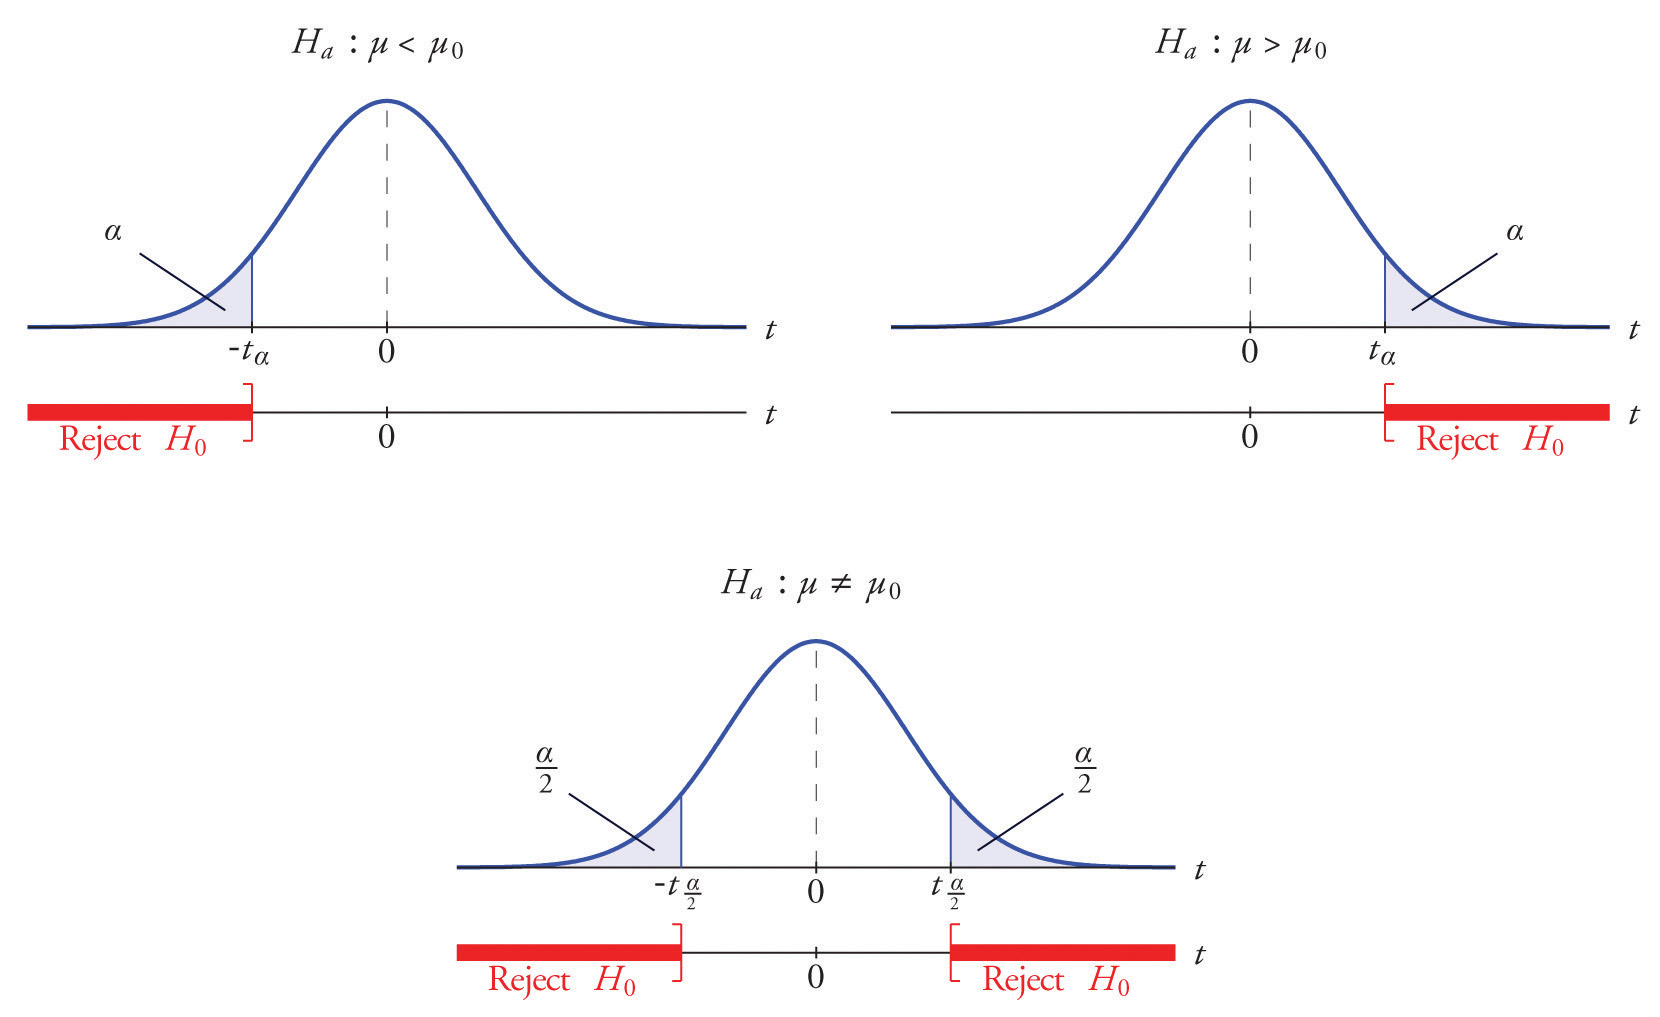
\includegraphics[width=.9\linewidth]{ht.jpg}
  \end{center}
\end{frame}

\begin{frame}{Type-1 and Type-2 error}
  \begin{table}
    \begin{tabular}{c|c|c}
      \toprule
      & \textbf{No reject} & \textbf{Reject} \\ \hline
      \textbf{$H_0$ true} & True Negative (TN) & {\color{blue} False Positive (FP)} \\
      & & {\color{blue} Type-1 error, $\alpha$} \\
      \textbf{$H_0$ false} & {\color{red} False Negative (FN)} & True Positive (TP) \\
      &  {\color{red}  Type-2 error, $\beta$} & \\
      \bottomrule
    \end{tabular}
  \end{table}
  \begin{center}
    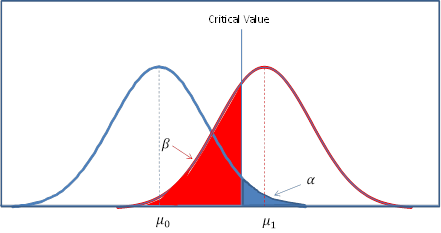
\includegraphics[width=.5\linewidth]{ht_error.png}
  \end{center}
\end{frame}

\begin{frame}{Overview hypothesis tests}
  \begin{table}
    \begin{tabular}{c|c|c}
      \toprule
      & \textbf{Discrete} & \textbf{Continuous} \\ \hline
      \textbf{Discrete} & Score test & Z test \\
      & Fisher's exact test & Student's t test \\
      & $\chi^2$ test & \\
      & Logistic regression & \\ \hline
      \textbf{Continuous} & \textit{Descretize} & Correlation \\
      &  & Linear regression \\
      \bottomrule
    \end{tabular}
  \end{table}
\end{frame}

\begin{frame}{p-value}
  \begin{center}
    \Large
    What is a p-value?
  \end{center}
\end{frame}

\begin{frame}{p-value}
  \begin{definition}[p-value]
    Probability to observe by chance a test statistic $T'$ that is at least as extreme as the observed test statistic $T_\mathcal{D}$, given that $H_0$ is true.
  \end{definition}
\end{frame}

\begin{frame}[fragile]{Testing two proportions}
  \begin{itemize}
    \item Are females more likely to develop T1D than males?
  \end{itemize}
  \begin{align*}
    X_f \sim \text{Bernoulli}(p_f) \quad X_m \sim \text{Bernoulli}(p_m)
  \end{align*}
  \begin{align*}
    H0: p_f = p_m
  \end{align*}
  \small
\begin{kframe}
\begin{alltt}
\hlstd{sex_t1d} \hlkwb{<-} \hlkwd{table}\hlstd{(t1d}\hlopt{$}\hlstd{sex,} \hlkwd{relevel}\hlstd{(t1d}\hlopt{$}\hlstd{t1d,} \hlstr{'yes'}\hlstd{))}
\hlkwd{xtable}\hlstd{(sex_t1d)}
\end{alltt}
\end{kframe}% latex table generated in R 3.1.1 by xtable 1.7-4 package
% Fri Nov 28 08:56:52 2014
\begin{table}[ht]
\centering
\begin{tabular}{rrr}
  \hline
 & yes & no \\ 
  \hline
f & 3775 & 946 \\ 
  m & 4086 & 820 \\ 
   \hline
\end{tabular}
\end{table}

\end{frame}

\begin{frame}[fragile]{Score test}
\begin{knitrout}\tiny
\definecolor{shadecolor}{rgb}{0.969, 0.969, 0.969}\color{fgcolor}\begin{kframe}
\begin{alltt}
\hlkwd{prop.test}\hlstd{(sex_t1d,} \hlkwc{conf.level}\hlstd{=}\hlnum{0.95}\hlstd{,} \hlkwc{alternative}\hlstd{=}\hlstr{'two.sided'}\hlstd{)}
\end{alltt}
\begin{verbatim}
## 
## 	2-sample test for equality of proportions with continuity
## 	correction
## 
## data:  sex_t1d
## X-squared = 17.524, df = 1, p-value = 2.837e-05
## alternative hypothesis: two.sided
## 95 percent confidence interval:
##  -0.04891865 -0.01755935
## sample estimates:
##    prop 1    prop 2 
## 0.7996187 0.8328577
\end{verbatim}
\end{kframe}
\end{knitrout}
  \begin{itemize}
    \item Depends on central limit theorem
    \item Requires many samples
  \end{itemize}
\end{frame}

\begin{frame}[fragile]{Fisher's exact test}
\begin{knitrout}\tiny
\definecolor{shadecolor}{rgb}{0.969, 0.969, 0.969}\color{fgcolor}\begin{kframe}
\begin{alltt}
\hlkwd{fisher.test}\hlstd{(sex_t1d,} \hlkwc{conf.level}\hlstd{=}\hlnum{0.95}\hlstd{,} \hlkwc{alternative}\hlstd{=}\hlstr{'two.sided'}\hlstd{)}
\end{alltt}
\begin{verbatim}
## 
## 	Fisher's Exact Test for Count Data
## 
## data:  sex_t1d
## p-value = 2.789e-05
## alternative hypothesis: true odds ratio is not equal to 1
## 95 percent confidence interval:
##  0.7210890 0.8893112
## sample estimates:
## odds ratio 
##   0.800854
\end{verbatim}
\end{kframe}
\end{knitrout}
  \begin{itemize}
    \item Does not depend on central limit theorem
    \item Does not require many samples
    \item Exact test: guarantees false positive rate
    \item Sometime too conservative
  \end{itemize}
\end{frame}

\begin{frame}[fragile]{Comparing means}
  \begin{itemize}
    \item Are females significantly older than males?
  \end{itemize}
  \begin{align*}
    X_f \sim \mathcal{N}(\mu_f, \sigma^2) \quad X_m \sim \mathcal{N}(\mu_m, \sigma^2)
  \end{align*}
  \begin{align*}
    H0: \mu_f < \mu_m
  \end{align*}
\begin{knitrout}\tiny
\definecolor{shadecolor}{rgb}{0.969, 0.969, 0.969}\color{fgcolor}\begin{kframe}
\begin{alltt}
\hlkwd{ggplot}\hlstd{(t1d)} \hlopt{+} \hlkwd{geom_density}\hlstd{(}\hlkwd{aes}\hlstd{(}\hlkwc{x}\hlstd{=age,} \hlkwc{y}\hlstd{=..density..,} \hlkwc{group}\hlstd{=sex,} \hlkwc{fill}\hlstd{=sex,} \hlkwc{color}\hlstd{=sex),} \hlkwc{alpha}\hlstd{=}\hlnum{.5}\hlstd{)}
\end{alltt}
\end{kframe}

{\centering \includegraphics[width=.8\linewidth]{figure/plot_age-1} 

}



\end{knitrout}
\end{frame}

\begin{frame}[fragile]{Student's t test}
\begin{knitrout}\tiny
\definecolor{shadecolor}{rgb}{0.969, 0.969, 0.969}\color{fgcolor}\begin{kframe}
\begin{alltt}
\hlkwd{t.test}\hlstd{(t1d}\hlopt{$}\hlstd{age[t1d}\hlopt{$}\hlstd{sex} \hlopt{==} \hlstr{'f'}\hlstd{], t1d}\hlopt{$}\hlstd{age[t1d}\hlopt{$}\hlstd{sex} \hlopt{==} \hlstr{'m'}\hlstd{],} \hlkwc{alternative}\hlstd{=}\hlstr{'greater'}\hlstd{)}
\end{alltt}
\begin{verbatim}
## 
## 	Welch Two Sample t-test
## 
## data:  t1d$age[t1d$sex == "f"] and t1d$age[t1d$sex == "m"]
## t = 1.644, df = 9594.183, p-value = 0.0501
## alternative hypothesis: true difference in means is greater than 0
## 95 percent confidence interval:
##  -7.709662e-05           Inf
## sample estimates:
## mean of x mean of y 
##  8.042441  7.911906
\end{verbatim}
\end{kframe}
\end{knitrout}
\end{frame}

\begin{frame}[fragile]{Testing dependency between variables}
  \begin{itemize}
    \item Does PTPN22 influence the risk of T1D?
  \end{itemize}
  \begin{align*}
    X_\text{PTPN22} \sim \text{Cat}(\{0, 1, 2\}) \quad
    X_\text{T1D} \sim \text{Bernoulli}(p)
  \end{align*}
  \begin{align*}
    H0: X_\text{PTPN22} \text{ independent of } X_\text{T1D}
  \end{align*}
\end{frame}

\begin{frame}[fragile]{Testing dependency between variables}
\begin{knitrout}\tiny
\definecolor{shadecolor}{rgb}{0.969, 0.969, 0.969}\color{fgcolor}\begin{kframe}
\begin{alltt}
\hlkwd{table}\hlstd{(t1d}\hlopt{$}\hlstd{ptpn22, t1d}\hlopt{$}\hlstd{t1d)}
\end{alltt}
\begin{verbatim}
##    
##       no  yes
##   0 1441 5381
##   1  313 2239
##   2   12  241
\end{verbatim}
\begin{alltt}
\hlkwd{ggplot}\hlstd{(t1d)} \hlopt{+} \hlkwd{geom_bar}\hlstd{(}\hlkwd{aes}\hlstd{(}\hlkwc{x}\hlstd{=ptpn22,} \hlkwc{fill}\hlstd{=t1d),} \hlkwc{position}\hlstd{=}\hlstr{'fill'}\hlstd{)} \hlopt{+}
\hlkwd{scale_x_discrete}\hlstd{(}\hlkwc{limits}\hlstd{=}\hlkwd{c}\hlstd{(}\hlnum{0}\hlstd{,} \hlnum{2}\hlstd{))} \hlopt{+} \hlkwd{xlab}\hlstd{(}\hlstr{'Risk level'}\hlstd{)} \hlopt{+} \hlkwd{ylab}\hlstd{(}\hlstr{'Proportion'}\hlstd{)}
\end{alltt}
\end{kframe}

{\centering \includegraphics[width=.6\linewidth]{figure/plot_ptpn22-1} 

}



\end{knitrout}
\end{frame}

\begin{frame}[fragile]{Testing dependency between variables}
  \begin{itemize}
    \item Fitting logistic regression model
  \end{itemize}
\begin{kframe}
\begin{alltt}
\hlstd{model} \hlkwb{<-} \hlkwd{glm}\hlstd{(t1d} \hlopt{~} \hlkwd{factor}\hlstd{(ptpn22),} \hlkwc{data}\hlstd{=t1d,} \hlkwc{family}\hlstd{=binomial)}
\hlkwd{xtable}\hlstd{(model)}
\end{alltt}
\end{kframe}% latex table generated in R 3.1.1 by xtable 1.7-4 package
% Fri Nov 28 08:56:52 2014
\begin{table}[ht]
\centering
\begin{tabular}{rrrrr}
  \hline
 & Estimate & Std. Error & z value & Pr($>$$|$z$|$) \\ 
  \hline
(Intercept) & 1.3175 & 0.0297 & 44.42 & 0.0000 \\ 
  factor(ptpn22)1 & 0.6500 & 0.0672 & 9.67 & 0.0000 \\ 
  factor(ptpn22)2 & 1.6824 & 0.2972 & 5.66 & 0.0000 \\ 
   \hline
\end{tabular}
\end{table}

\end{frame}

\begin{frame}[fragile]{Testing dependency between variables}
  \begin{itemize}
    \item Likelihood Ratio Test
  \end{itemize}
\begin{knitrout}\tiny
\definecolor{shadecolor}{rgb}{0.969, 0.969, 0.969}\color{fgcolor}\begin{kframe}
\begin{alltt}
\hlkwd{anova}\hlstd{(model,} \hlkwc{test}\hlstd{=}\hlstr{'LRT'}\hlstd{)}
\end{alltt}
\begin{verbatim}
## Analysis of Deviance Table
## 
## Model: binomial, link: logit
## 
## Response: t1d
## 
## Terms added sequentially (first to last)
## 
## 
##                Df Deviance Resid. Df Resid. Dev  Pr(>Chi)    
## NULL                            9626     9175.9              
## factor(ptpn22)  2   145.24      9624     9030.7 < 2.2e-16 ***
## ---
## Signif. codes:  0 '***' 0.001 '**' 0.01 '*' 0.05 '.' 0.1 ' ' 1
\end{verbatim}
\end{kframe}
\end{knitrout}
\end{frame}

\begin{frame}[fragile]{Testing dependency between variables}
  \begin{itemize}
    \item Does PTPN22 influence the risk of T1D, accounting for all other
      variables?
  \end{itemize}
  \begin{align*}
    X_\text{PTPN22} \sim \text{Cat}(\{0, 1, 2\}) \quad
    X_\text{T1D} \sim \text{Bernoulli}(p)
  \end{align*}
  \begin{align*}
    H0: X_\text{PTPN22} \text{ independent of } X_\text{T1D} 
    \text{, accounting for } X_\text{age}, X_\text{ERBB3}, X_\text{IL10}, \dots
  \end{align*}
\end{frame}

\begin{frame}[fragile]{Testing dependency between variables}
  \begin{itemize}
    \item Fitting logistic regression model
  \end{itemize}
\begin{kframe}
\begin{alltt}
\hlstd{model} \hlkwb{<-} \hlkwd{glm}\hlstd{(t1d} \hlopt{~} \hlstd{.}\hlopt{-}\hlstd{(european),} \hlkwc{data}\hlstd{=t1d,} \hlkwc{family}\hlstd{=binomial)}
\hlkwd{xtable}\hlstd{(model)}
\end{alltt}
\end{kframe}% latex table generated in R 3.1.1 by xtable 1.7-4 package
% Fri Nov 28 08:55:04 2014
\begin{table}[ht]
\centering
\begin{tabular}{rrrrr}
  \hline
 & Estimate & Std. Error & z value & Pr($>$$|$z$|$) \\ 
  \hline
(Intercept) & -2.2612 & 0.1583 & -14.29 & 0.0000 \\ 
  hlacat & 0.8121 & 0.0240 & 33.89 & 0.0000 \\ 
  sexm & 0.1896 & 0.0601 & 3.16 & 0.0016 \\ 
  age & 0.0151 & 0.0077 & 1.95 & 0.0512 \\ 
  ptpn22 & 0.7633 & 0.0673 & 11.34 & 0.0000 \\ 
  il10 & 0.2665 & 0.0585 & 4.56 & 0.0000 \\ 
  ctla4 & 0.0788 & 0.0431 & 1.83 & 0.0675 \\ 
  bach2 & 0.2285 & 0.0422 & 5.42 & 0.0000 \\ 
  erbb3 & 0.3360 & 0.0447 & 7.52 & 0.0000 \\ 
  gab3 & 0.1930 & 0.0374 & 5.16 & 0.0000 \\ 
   \hline
\end{tabular}
\end{table}

\end{frame}

\begin{frame}[fragile]{Testing dependency between variables}
\begin{knitrout}\tiny
\definecolor{shadecolor}{rgb}{0.969, 0.969, 0.969}\color{fgcolor}\begin{kframe}
\begin{alltt}
\hlstd{lor} \hlkwb{<-} \hlkwd{sort}\hlstd{(}\hlkwd{coef}\hlstd{(model)[}\hlopt{-}\hlnum{1}\hlstd{],} \hlkwc{decreasing}\hlstd{=}\hlnum{TRUE}\hlstd{)}
\hlkwd{barplot}\hlstd{(lor,} \hlkwc{las}\hlstd{=}\hlnum{2}\hlstd{,} \hlkwc{col}\hlstd{=}\hlstr{'lightblue'}\hlstd{,} \hlkwc{ylab}\hlstd{=}\hlstr{'Log-odds ratio'}\hlstd{)}
\end{alltt}
\end{kframe}

{\centering \includegraphics[width=.9\linewidth]{figure/glm_all_lor-1} 

}



\end{knitrout}
\end{frame}


\section{Clustering}
\begin{frame}
\tableofcontents[currentsection]
\end{frame}

\begin{frame}[fragile]{Clustering}
  \begin{columns}
    \begin{column}{.5\linewidth}
      \begin{itemize}
        \item \textbf{Goal}: Finding groups of related items
          \vspace{1cm}
        \item How do define relatedness?
        \item Which clustering methods exist?
        \item What is Hierarchical clustering?
        \item How to visualize clustering?
      \end{itemize}
    \end{column}
    \begin{column}{.5\linewidth}
      \begin{center}
        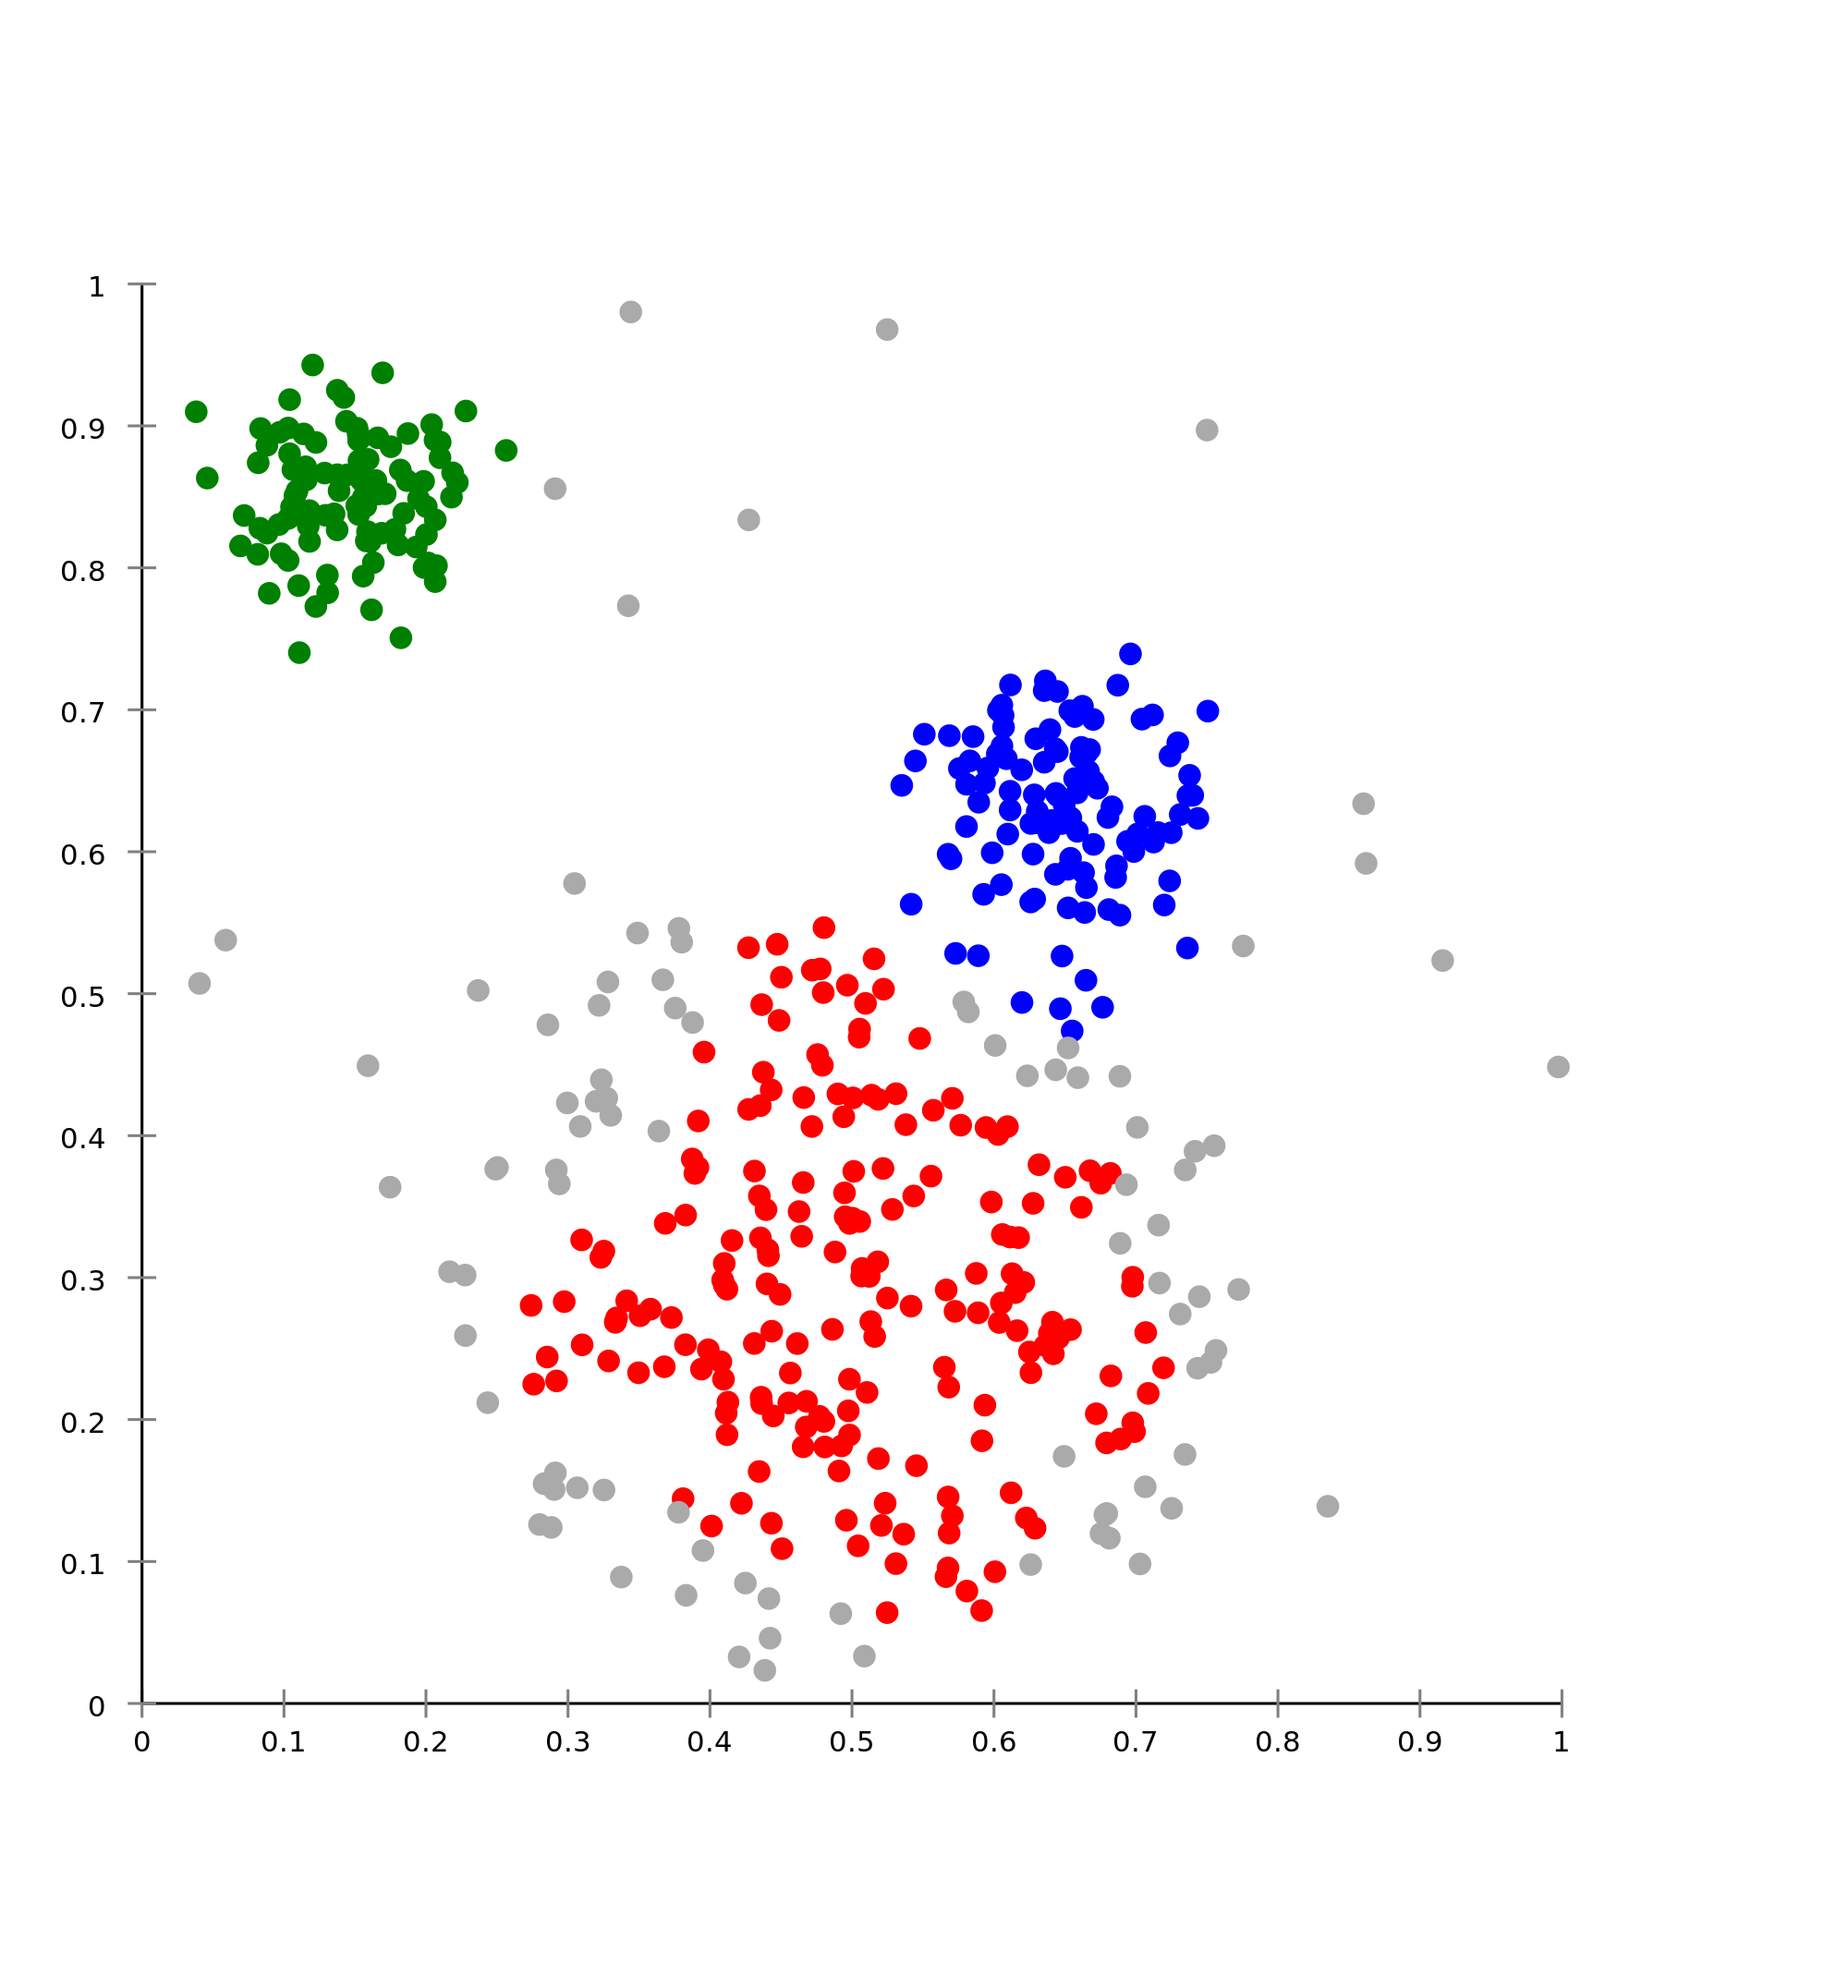
\includegraphics[width=.8\linewidth]{clust.png}
      \end{center}
    \end{column}
  \end{columns}
\end{frame}

\begin{frame}[fragile]{How to define relatedness?}
  \begin{block}{Distance}
    \begin{itemize}
      \item Euclidean distance
      \item Manhattan distance
      \item Binary distance
    \end{itemize}
  \end{block}
  \begin{block}{Similarity}
    \begin{itemize}
      \item Identity
      \item Correlation
        \vspace{.3cm}
      \item $\rightarrow$ Every similarity can be converted into distance
    \end{itemize}
  \end{block}
\end{frame}

\begin{frame}[fragile]{Euclidean distance}
  \begin{columns}
    \begin{column}{.5\linewidth}
      \begin{Definition}{Euclidean distance}
        \begin{align*}
          d(x, y) = \sqrt{\sum_i (x_i - y_i)^2}
        \end{align*}
      \end{Definition}
    \end{column}
    \begin{column}{.5\linewidth}
      \begin{center}
        \includegraphics[width=.8\linewidth]{dist_eucl.pdf}
      \end{center}
    \end{column}
  \end{columns}
\end{frame}

\begin{frame}[fragile]{Manhattan distance}
  \begin{columns}
    \begin{column}{.5\linewidth}
      \begin{Definition}{Manhattan distance}
        \begin{align*}
          d(x, y) = \sum_i |x_i - y_i|
        \end{align*}
      \end{Definition}
    \end{column}
    \begin{column}{.5\linewidth}
      \begin{center}
        \includegraphics[width=.8\linewidth]{dist_man.pdf}
      \end{center}
    \end{column}
  \end{columns}
\end{frame}

\begin{frame}[fragile]{Methods}
  \begin{columns}[t]
    \begin{column}{.32\linewidth}
      \begin{block}{Partitioning clustering}
        \only<2->{
        \begin{itemize}
          \item Partition points into k clusters
          \item k known a-priori
          \item k-means
          \item k-medoids
        \end{itemize}
        \begin{center}
          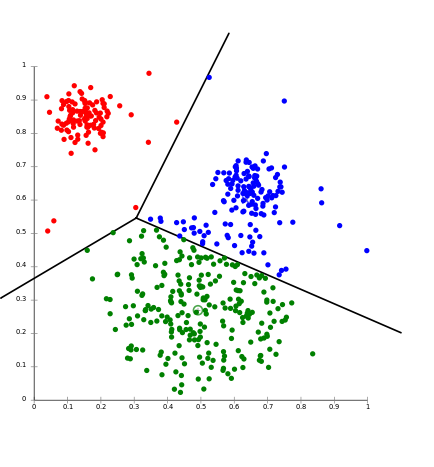
\includegraphics[width=\linewidth]{clust_part.png}
        \end{center}}
      \end{block}
    \end{column}
    \begin{column}{.32\linewidth}
      \begin{block}{Density clustering}
        \only<3->{
        \begin{itemize}
          \item Cluster points into dense regions
          \item k unknown a-priori
          \item DBSCAN
          \item OPTICS
        \end{itemize}
        \begin{center}
          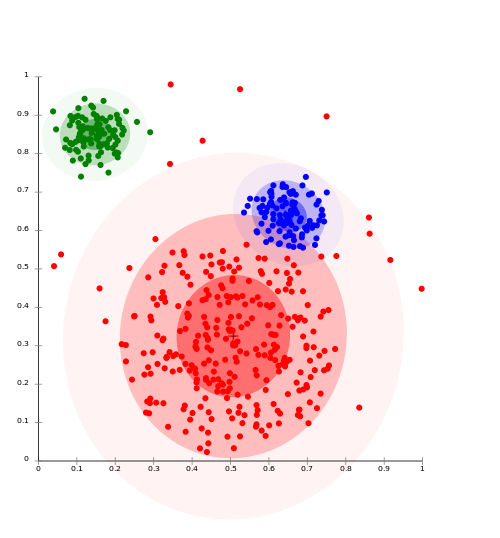
\includegraphics[width=\linewidth]{clust_dens.png}
        \end{center}}
      \end{block}
    \end{column}
    \begin{column}{.32\linewidth}
      \begin{block}{Hierarchical clustering}
        \only<4->{
        \begin{itemize}
          \item Find hierarchy of clusters
          \item k unknown a-priori
          \item Single-linkage
          \item Complete-linkage
          \item Average-linkage
        \end{itemize}
        \begin{center}
          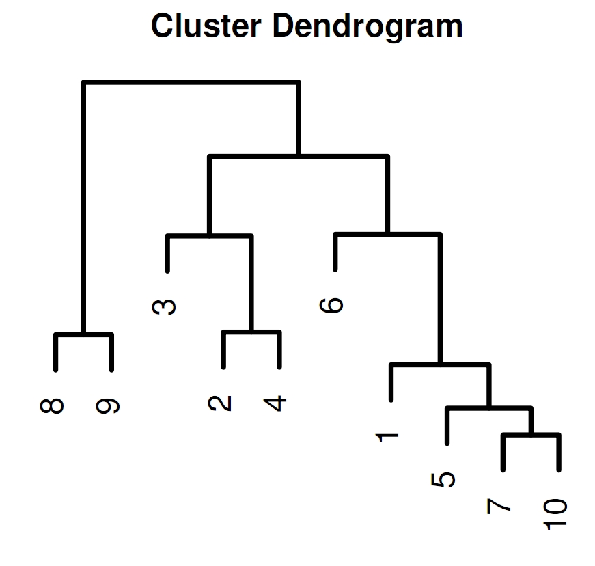
\includegraphics[width=.7\linewidth]{clust_hier.png}
        \end{center}}
      \end{block}
    \end{column}
  \end{columns}
\end{frame}

\begin{frame}[fragile]{Hierarchical clustering}
  \begin{itemize}
    \item Constructs hierarchy of clusters represented by a \alert{Cluster dendrogram}
    \item \alert{Cluster dendrogram}
      \begin{itemize}
        \item Leaf nodes: single data points
        \item Inner nodes: cluster of points
        \item Root node: all data points
      \end{itemize}
  \end{itemize}
  \begin{center}
    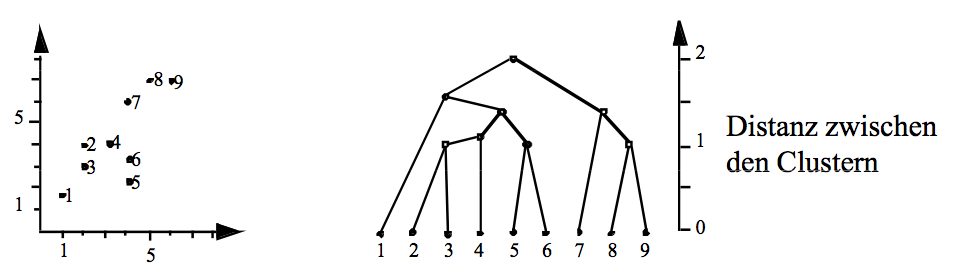
\includegraphics[width=.8\linewidth]{clust_dendro.png}
  \end{center}
\end{frame}

\begin{frame}[fragile]{Algorithm}
  \begin{enumerate}
    \item Start with clusters that contain only one point
    \item Compute distance between clusters
    \item Merge the two clusters with lowest distance into new cluster
    \item Go to step 2 until one single cluster remains
  \end{enumerate}
\end{frame}

\begin{frame}[fragile]{How to compute the distance between clusters?}
  \begin{center}
    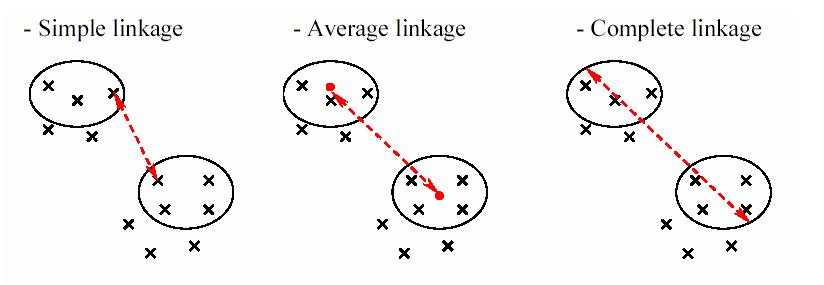
\includegraphics[width=\linewidth]{clust_linkage.jpg}
  \end{center}
\end{frame}



\begin{frame}[fragile]{Data}
\begin{knitrout}\tiny
\definecolor{shadecolor}{rgb}{0.969, 0.969, 0.969}\color{fgcolor}\begin{kframe}
\begin{alltt}
\hlkwd{set.seed}\hlstd{(}\hlnum{5}\hlstd{)}
\hlstd{n} \hlkwb{=} \hlnum{5}
\hlstd{nclust} \hlkwb{=} \hlnum{3}
\hlstd{x_means} \hlkwb{=} \hlkwd{c}\hlstd{(}\hlnum{1}\hlstd{,} \hlnum{2}\hlstd{,} \hlnum{2.5}\hlstd{)}
\hlstd{y_means} \hlkwb{=} \hlkwd{c}\hlstd{(}\hlnum{1}\hlstd{,} \hlnum{2.5}\hlstd{,} \hlnum{2}\hlstd{)}
\hlstd{x} \hlkwb{=} \hlkwd{rnorm}\hlstd{(n} \hlopt{*} \hlstd{nclust,} \hlkwd{rep}\hlstd{(x_means,} \hlkwc{each}\hlstd{=n),} \hlkwc{sd}\hlstd{=}\hlnum{.4}\hlstd{)}
\hlstd{y} \hlkwb{=} \hlkwd{rnorm}\hlstd{(n} \hlopt{*} \hlstd{nclust,} \hlkwd{rep}\hlstd{(y_means,} \hlkwc{each}\hlstd{=n),} \hlkwc{sd}\hlstd{=}\hlnum{.4}\hlstd{)}
\hlstd{clust} \hlkwb{=} \hlkwd{factor}\hlstd{(}\hlkwd{rep}\hlstd{(}\hlnum{1}\hlopt{:}\hlstd{nclust,} \hlkwc{each}\hlstd{=n))}
\hlstd{id} \hlkwb{=} \hlnum{1}\hlopt{:}\hlstd{(n} \hlopt{*} \hlstd{nclust)}
\hlstd{cdata} \hlkwb{=} \hlkwd{data.frame}\hlstd{(}\hlkwc{id}\hlstd{=id,} \hlkwc{x}\hlstd{=x,} \hlkwc{y}\hlstd{=y,} \hlkwc{clust}\hlstd{=clust)}
\hlkwd{ggplot}\hlstd{(cdata,} \hlkwd{aes}\hlstd{(}\hlkwc{x}\hlstd{=x,} \hlkwc{y}\hlstd{=y))} \hlopt{+} \hlkwd{geom_point}\hlstd{(}\hlkwd{aes}\hlstd{(}\hlkwc{color}\hlstd{=clust),} \hlkwc{size}\hlstd{=}\hlnum{3}\hlstd{,} \hlkwc{show_guide}\hlstd{=F)} \hlopt{+}
  \hlkwd{geom_text}\hlstd{(}\hlkwd{aes}\hlstd{(}\hlkwc{label}\hlstd{=id,} \hlkwc{color}\hlstd{=clust),} \hlkwc{show_guide}\hlstd{=F,} \hlkwc{vjust}\hlstd{=}\hlopt{-}\hlnum{.3}\hlstd{,} \hlkwc{hjust}\hlstd{=}\hlnum{0}\hlstd{)}
\end{alltt}
\end{kframe}

{\centering \includegraphics[width=.6\linewidth]{figure/clust_data-1} 

}



\end{knitrout}
\end{frame}

\begin{frame}[fragile]{Data}
\begin{knitrout}\tiny
\definecolor{shadecolor}{rgb}{0.969, 0.969, 0.969}\color{fgcolor}\begin{kframe}
\begin{alltt}
\hlkwd{set.seed}\hlstd{(}\hlnum{5}\hlstd{)}
\hlstd{n} \hlkwb{=} \hlnum{5}
\hlstd{nclust} \hlkwb{=} \hlnum{3}
\hlstd{x_means} \hlkwb{=} \hlkwd{c}\hlstd{(}\hlnum{1}\hlstd{,} \hlnum{2}\hlstd{,} \hlnum{2.5}\hlstd{)}
\hlstd{y_means} \hlkwb{=} \hlkwd{c}\hlstd{(}\hlnum{1}\hlstd{,} \hlnum{2.5}\hlstd{,} \hlnum{2}\hlstd{)}
\hlstd{x} \hlkwb{=} \hlkwd{rnorm}\hlstd{(n} \hlopt{*} \hlstd{nclust,} \hlkwd{rep}\hlstd{(x_means,} \hlkwc{each}\hlstd{=n),} \hlkwc{sd}\hlstd{=}\hlnum{.4}\hlstd{)}
\hlstd{y} \hlkwb{=} \hlkwd{rnorm}\hlstd{(n} \hlopt{*} \hlstd{nclust,} \hlkwd{rep}\hlstd{(y_means,} \hlkwc{each}\hlstd{=n),} \hlkwc{sd}\hlstd{=}\hlnum{.4}\hlstd{)}
\hlstd{clust} \hlkwb{=} \hlkwd{factor}\hlstd{(}\hlkwd{rep}\hlstd{(}\hlnum{1}\hlopt{:}\hlstd{nclust,} \hlkwc{each}\hlstd{=n))}
\hlstd{id} \hlkwb{=} \hlnum{1}\hlopt{:}\hlstd{(n} \hlopt{*} \hlstd{nclust)}
\hlstd{cdata} \hlkwb{=} \hlkwd{data.frame}\hlstd{(}\hlkwc{id}\hlstd{=id,} \hlkwc{x}\hlstd{=x,} \hlkwc{y}\hlstd{=y,} \hlkwc{clust}\hlstd{=clust)}
\hlkwd{ggplot}\hlstd{(cdata,} \hlkwd{aes}\hlstd{(}\hlkwc{x}\hlstd{=x,} \hlkwc{y}\hlstd{=y))} \hlopt{+} \hlkwd{geom_point}\hlstd{(}\hlkwc{color}\hlstd{=}\hlstr{'black'}\hlstd{,} \hlkwc{size}\hlstd{=}\hlnum{3}\hlstd{,} \hlkwc{show_guide}\hlstd{=F)} \hlopt{+}
  \hlkwd{geom_text}\hlstd{(}\hlkwd{aes}\hlstd{(}\hlkwc{label}\hlstd{=id),} \hlkwc{color}\hlstd{=}\hlstr{'black'}\hlstd{,} \hlkwc{show_guide}\hlstd{=F,} \hlkwc{vjust}\hlstd{=}\hlopt{-}\hlnum{.3}\hlstd{,} \hlkwc{hjust}\hlstd{=}\hlnum{0}\hlstd{)}
\end{alltt}
\end{kframe}

{\centering \includegraphics[width=.6\linewidth]{figure/clust_data_black-1} 

}



\end{knitrout}
\end{frame}

\begin{frame}[fragile]{Complete linkage}
\begin{knitrout}\tiny
\definecolor{shadecolor}{rgb}{0.969, 0.969, 0.969}\color{fgcolor}\begin{kframe}
\begin{alltt}
\hlstd{cdist} \hlkwb{=} \hlkwd{dist}\hlstd{(}\hlkwd{cbind}\hlstd{(cdata}\hlopt{$}\hlstd{x, cdata}\hlopt{$}\hlstd{y),} \hlkwc{method}\hlstd{=}\hlstr{'euclidean'}\hlstd{)}
\hlstd{chclust} \hlkwb{=} \hlkwd{hclust}\hlstd{(cdist,} \hlkwc{method}\hlstd{=}\hlstr{'complete'}\hlstd{)}
\hlkwd{plot}\hlstd{(chclust,} \hlkwc{ylab}\hlstd{=}\hlstr{'Distance'}\hlstd{,} \hlkwc{xlab}\hlstd{=}\hlnum{NA}\hlstd{,} \hlkwc{main}\hlstd{=}\hlnum{NA}\hlstd{,} \hlkwc{sub}\hlstd{=}\hlnum{NA}\hlstd{)}
\end{alltt}
\end{kframe}

{\centering \includegraphics[width=.8\linewidth]{figure/clust_complete-1} 

}



\end{knitrout}
\end{frame}

\begin{frame}[fragile]{Average linkage}
\begin{knitrout}\tiny
\definecolor{shadecolor}{rgb}{0.969, 0.969, 0.969}\color{fgcolor}\begin{kframe}
\begin{alltt}
\hlstd{cdist} \hlkwb{=} \hlkwd{dist}\hlstd{(}\hlkwd{cbind}\hlstd{(cdata}\hlopt{$}\hlstd{x, cdata}\hlopt{$}\hlstd{y),} \hlkwc{method}\hlstd{=}\hlstr{'euclidean'}\hlstd{)}
\hlstd{chclust} \hlkwb{=} \hlkwd{hclust}\hlstd{(cdist,} \hlkwc{method}\hlstd{=}\hlstr{'average'}\hlstd{)}
\hlkwd{plot}\hlstd{(chclust,} \hlkwc{ylab}\hlstd{=}\hlstr{'Distance'}\hlstd{,} \hlkwc{xlab}\hlstd{=}\hlnum{NA}\hlstd{,} \hlkwc{main}\hlstd{=}\hlnum{NA}\hlstd{,} \hlkwc{sub}\hlstd{=}\hlnum{NA}\hlstd{)}
\end{alltt}
\end{kframe}

{\centering \includegraphics[width=.8\linewidth]{figure/clust_average-1} 

}



\end{knitrout}
\end{frame}

\begin{frame}[fragile]{Single linkage}
\begin{knitrout}\tiny
\definecolor{shadecolor}{rgb}{0.969, 0.969, 0.969}\color{fgcolor}\begin{kframe}
\begin{alltt}
\hlstd{cdist} \hlkwb{=} \hlkwd{dist}\hlstd{(}\hlkwd{cbind}\hlstd{(cdata}\hlopt{$}\hlstd{x, cdata}\hlopt{$}\hlstd{y),} \hlkwc{method}\hlstd{=}\hlstr{'euclidean'}\hlstd{)}
\hlstd{chclust} \hlkwb{=} \hlkwd{hclust}\hlstd{(cdist,} \hlkwc{method}\hlstd{=}\hlstr{'single'}\hlstd{)}
\hlkwd{plot}\hlstd{(chclust,} \hlkwc{ylab}\hlstd{=}\hlstr{'Distance'}\hlstd{,} \hlkwc{xlab}\hlstd{=}\hlnum{NA}\hlstd{,} \hlkwc{main}\hlstd{=}\hlnum{NA}\hlstd{,} \hlkwc{sub}\hlstd{=}\hlnum{NA}\hlstd{)}
\end{alltt}
\end{kframe}

{\centering \includegraphics[width=.8\linewidth]{figure/clust_single-1} 

}



\end{knitrout}
\end{frame}

\begin{frame}[fragile]{Data}
\begin{knitrout}\tiny
\definecolor{shadecolor}{rgb}{0.969, 0.969, 0.969}\color{fgcolor}\begin{kframe}
\begin{alltt}
\hlkwd{set.seed}\hlstd{(}\hlnum{5}\hlstd{)}
\hlstd{n} \hlkwb{=} \hlnum{5}
\hlstd{nclust} \hlkwb{=} \hlnum{3}
\hlstd{x_means} \hlkwb{=} \hlkwd{c}\hlstd{(}\hlnum{1}\hlstd{,} \hlnum{2}\hlstd{,} \hlnum{2.5}\hlstd{)}
\hlstd{y_means} \hlkwb{=} \hlkwd{c}\hlstd{(}\hlnum{1}\hlstd{,} \hlnum{2.5}\hlstd{,} \hlnum{2}\hlstd{)}
\hlstd{x} \hlkwb{=} \hlkwd{rnorm}\hlstd{(n} \hlopt{*} \hlstd{nclust,} \hlkwd{rep}\hlstd{(x_means,} \hlkwc{each}\hlstd{=n),} \hlkwc{sd}\hlstd{=}\hlnum{.4}\hlstd{)}
\hlstd{y} \hlkwb{=} \hlkwd{rnorm}\hlstd{(n} \hlopt{*} \hlstd{nclust,} \hlkwd{rep}\hlstd{(y_means,} \hlkwc{each}\hlstd{=n),} \hlkwc{sd}\hlstd{=}\hlnum{.4}\hlstd{)}
\hlstd{clust} \hlkwb{=} \hlkwd{factor}\hlstd{(}\hlkwd{rep}\hlstd{(}\hlnum{1}\hlopt{:}\hlstd{nclust,} \hlkwc{each}\hlstd{=n))}
\hlstd{id} \hlkwb{=} \hlnum{1}\hlopt{:}\hlstd{(n} \hlopt{*} \hlstd{nclust)}
\hlstd{cdata} \hlkwb{=} \hlkwd{data.frame}\hlstd{(}\hlkwc{id}\hlstd{=id,} \hlkwc{x}\hlstd{=x,} \hlkwc{y}\hlstd{=y,} \hlkwc{clust}\hlstd{=clust)}
\hlkwd{ggplot}\hlstd{(cdata,} \hlkwd{aes}\hlstd{(}\hlkwc{x}\hlstd{=x,} \hlkwc{y}\hlstd{=y))} \hlopt{+} \hlkwd{geom_point}\hlstd{(}\hlkwd{aes}\hlstd{(}\hlkwc{color}\hlstd{=clust),} \hlkwc{size}\hlstd{=}\hlnum{3}\hlstd{,} \hlkwc{show_guide}\hlstd{=F)} \hlopt{+}
  \hlkwd{geom_text}\hlstd{(}\hlkwd{aes}\hlstd{(}\hlkwc{label}\hlstd{=id,} \hlkwc{color}\hlstd{=clust),} \hlkwc{show_guide}\hlstd{=F,} \hlkwc{vjust}\hlstd{=}\hlopt{-}\hlnum{.3}\hlstd{,} \hlkwc{hjust}\hlstd{=}\hlnum{0}\hlstd{)}
\end{alltt}
\end{kframe}

{\centering \includegraphics[width=.6\linewidth]{figure/clust_data2-1} 

}



\end{knitrout}
\end{frame}

\section{PCA}
\begin{frame}
\tableofcontents[currentsection]
\end{frame}

\begin{frame}{High-dimensional data}
  \begin{itemize}
    \item \alert{Small $n$ large $p$}
    \item Few samples $n$ ($\approx 100$)
    \item Many features $p$
      \begin{itemize}
        \item $> 10000$ genes
        \item $> 27000000$ CpG sites
      \end{itemize}
  \end{itemize}
  \begin{center}
    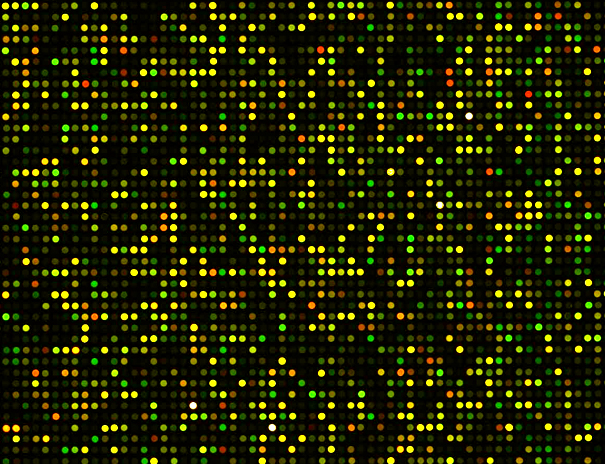
\includegraphics[width=.5\linewidth]{microarray.jpg}
  \end{center}
\end{frame}

\begin{frame}{Problems}
  \begin{itemize}
    \item High storage costs (memory)
    \item High computational costs (time)
    \item Visualization?
    \item Curse of dimensionality
  \end{itemize}
  \begin{center}
    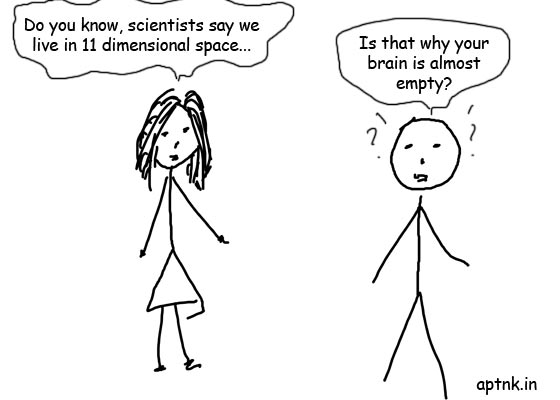
\includegraphics[width=.5\linewidth]{curse_dim.jpg}
  \end{center}
\end{frame}

\begin{frame}{Principle Component Analysis}
  \begin{itemize}
    \item Dimensionality reduction
    \item Visualization
    \item Missing values imputation
    \item Latent factors estimation:
      \begin{itemize}
        \item Population structure
        \item Batch-effects
        \item Cell-cycle
      \end{itemize}
  \end{itemize}
\end{frame}

\begin{frame}{Principle components}
  \begin{itemize}
    \item Minimize projection error
    \item Maximize variance
  \end{itemize}
  \begin{center}
    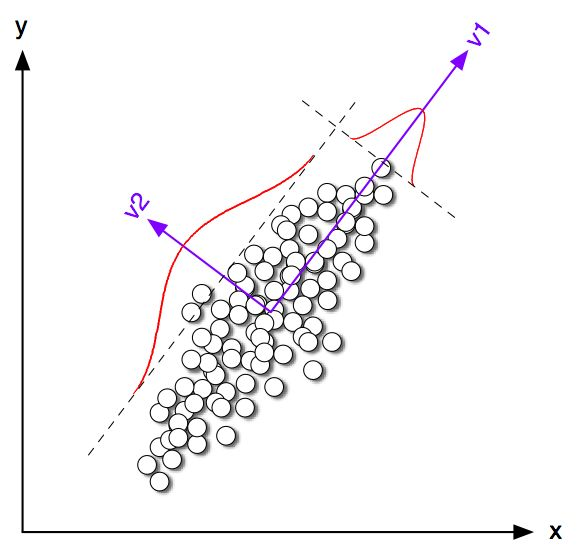
\includegraphics[width=.6\linewidth]{pca.jpg}
  \end{center}
\end{frame}

\begin{frame}{Pearson correlation coefficient}
  \begin{itemize}
    \item Measures \textbf{linear} dependency between $x$ and $y$
    \item $cor(x,y) = \in \left[-1,+1\right]$
    \item $cor(x,y) = 0$: no correlation
    \item $cor(x,y) = -1$: negative correlation
    \item $cor(x,y) = +1$: positive correlation
  \end{itemize}
  \begin{definition}[Pearson correlation coefficient]
    \begin{align*}
      \operatorname{cor}(x, y) = \frac{\sum_i (x_i - \bar{x})(y_i - \bar{y})}
      {\sqrt{\sum_i (x_i - \bar{x})^2}\sqrt{\sum_i (y_i - \bar{y})^2}}
    \end{align*}
  \end{definition}
\end{frame}

\begin{frame}{Pearson correlation coefficient}
  \begin{center}
    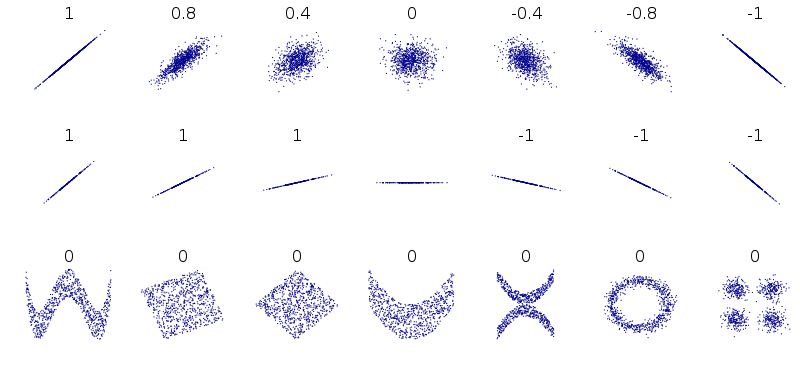
\includegraphics[width=0.8\linewidth]{pearson.png}
  \end{center}
\end{frame}

\begin{frame}{Spearman correlation coefficient}
  \begin{itemize}
    \item Measures \textbf{monotonic} dependency between $x$ and $y$
    \item Pearson correlation coefficient on rank of variables
    \item $cor(x,y) = \in \left[-1,+1\right]$
  \end{itemize}
  \begin{center}
    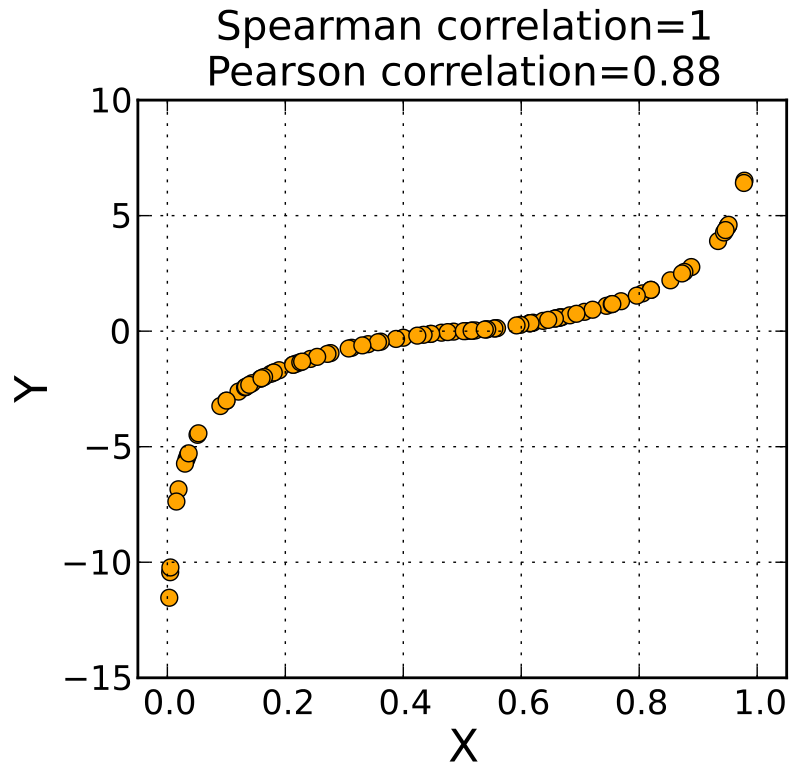
\includegraphics[width=0.4\linewidth]{spearman.png}
  \end{center}
\end{frame}



\begin{frame}[fragile]{Embryonic Stem Cell (ESC) data}
  \begin{itemize}
    \item Single-cell RNA-seq
    \item $n=182$ Embryonic stem cells
    \item $p=9571$ Genes
    \item Cell-cycle via Hoechst staining
  \end{itemize}
\begin{knitrout}\tiny
\definecolor{shadecolor}{rgb}{0.969, 0.969, 0.969}\color{fgcolor}

{\centering \includegraphics[width=.9\linewidth]{figure/heat_esc-1} 

}



\end{knitrout}
\end{frame}

\begin{frame}[fragile]{Correlation between two ESC}
\begin{knitrout}\tiny
\definecolor{shadecolor}{rgb}{0.969, 0.969, 0.969}\color{fgcolor}\begin{kframe}
\begin{alltt}
\hlstd{c1} \hlkwb{<-} \hlstd{esc}\hlopt{$}\hlstd{counts[}\hlkwd{which}\hlstd{(esc}\hlopt{$}\hlstd{cycle} \hlopt{==} \hlstr{'G1'}\hlstd{)[}\hlnum{1}\hlstd{],]}
\hlstd{c2} \hlkwb{<-} \hlstd{esc}\hlopt{$}\hlstd{counts[}\hlkwd{which}\hlstd{(esc}\hlopt{$}\hlstd{cycle} \hlopt{==} \hlstr{'S'}\hlstd{)[}\hlnum{1}\hlstd{],]}
\end{alltt}
\end{kframe}
\end{knitrout}
  \begin{columns}[c]
    \begin{column}{.5\linewidth}
\begin{knitrout}\tiny
\definecolor{shadecolor}{rgb}{0.969, 0.969, 0.969}\color{fgcolor}\begin{kframe}
\begin{alltt}
\hlkwd{qplot}\hlstd{(c1, c2,} \hlkwc{xlab}\hlstd{=}\hlstr{'G1 cell'}\hlstd{,} \hlkwc{ylab}\hlstd{=}\hlstr{'S cell'}\hlstd{)}
\end{alltt}
\end{kframe}

{\centering \includegraphics[width=\linewidth]{figure/cor_c1_c2-1} 

}



\end{knitrout}
    \end{column}
    \begin{column}{.5\linewidth}
\begin{knitrout}\tiny
\definecolor{shadecolor}{rgb}{0.969, 0.969, 0.969}\color{fgcolor}\begin{kframe}
\begin{alltt}
\hlkwd{cor}\hlstd{(c1, c2,}
    \hlkwc{method}\hlstd{=}\hlstr{'pearson'}\hlstd{)}
\end{alltt}
\begin{verbatim}
## [1] 0.547453
\end{verbatim}
\begin{alltt}
\hlkwd{cor}\hlstd{(c1, c2,}
    \hlkwc{method}\hlstd{=}\hlstr{'spearman'}\hlstd{)}
\end{alltt}
\begin{verbatim}
## [1] 0.5785747
\end{verbatim}
\end{kframe}
\end{knitrout}
    \end{column}
  \end{columns}
\end{frame}

\begin{frame}[fragile]{Correlation matrix}
\begin{knitrout}\tiny
\definecolor{shadecolor}{rgb}{0.969, 0.969, 0.969}\color{fgcolor}\begin{kframe}
\begin{alltt}
\hlstd{cor_cells} \hlkwb{<-} \hlkwd{cor}\hlstd{(}\hlkwd{t}\hlstd{(esc}\hlopt{$}\hlstd{counts),} \hlkwc{method}\hlstd{=}\hlstr{'pearson'}\hlstd{)}
\hlkwd{heatmap}\hlstd{(cor_cells,} \hlkwc{Rowv}\hlstd{=}\hlnum{NA}\hlstd{,} \hlkwc{Colv}\hlstd{=}\hlnum{NA}\hlstd{)}
\end{alltt}
\end{kframe}

{\centering \includegraphics[width=.5\linewidth]{figure/cor_matrix-1} 

}



\end{knitrout}
\end{frame}

\begin{frame}[fragile]{PCA}
\begin{knitrout}\tiny
\definecolor{shadecolor}{rgb}{0.969, 0.969, 0.969}\color{fgcolor}\begin{kframe}
\begin{alltt}
\hlstd{svd} \hlkwb{<-} \hlkwd{svd}\hlstd{(}\hlkwd{scale}\hlstd{(esc}\hlopt{$}\hlstd{counts))}
\hlstd{dsvd} \hlkwb{<-} \hlkwd{as.data.frame}\hlstd{(svd}\hlopt{$}\hlstd{u[,} \hlnum{1}\hlopt{:}\hlnum{10}\hlstd{])}
\hlkwd{colnames}\hlstd{(dsvd)} \hlkwb{<-} \hlkwd{paste0}\hlstd{(}\hlstr{'pc'}\hlstd{,} \hlkwd{seq}\hlstd{(}\hlnum{1}\hlstd{,} \hlkwd{ncol}\hlstd{(dsvd)))}
\hlstd{dsvd}\hlopt{$}\hlstd{cycle} \hlkwb{<-} \hlstd{esc}\hlopt{$}\hlstd{cycle}
\hlstd{ve} \hlkwb{<-} \hlstd{svd}\hlopt{$}\hlstd{d}\hlopt{^}\hlnum{2} \hlopt{/} \hlkwd{sum}\hlstd{(svd}\hlopt{$}\hlstd{d}\hlopt{^}\hlnum{2}\hlstd{)}
\hlkwd{barplot}\hlstd{(ve[}\hlnum{1}\hlopt{:}\hlnum{10}\hlstd{],} \hlkwc{xlab}\hlstd{=}\hlstr{'Principle components'}\hlstd{,} \hlkwc{ylab}\hlstd{=}\hlstr{'% Variance explained'}\hlstd{,}
        \hlkwc{col}\hlstd{=}\hlstr{'lightblue'}\hlstd{)}
\end{alltt}
\end{kframe}

{\centering \includegraphics[width=.8\linewidth]{figure/pca_ve-1} 

}



\end{knitrout}
\end{frame}

\begin{frame}[fragile]{PC1 versus PC2}
\begin{knitrout}\tiny
\definecolor{shadecolor}{rgb}{0.969, 0.969, 0.969}\color{fgcolor}\begin{kframe}
\begin{alltt}
\hlkwd{ggplot}\hlstd{(dsvd,} \hlkwd{aes}\hlstd{(}\hlkwc{x}\hlstd{=pc1,} \hlkwc{y}\hlstd{=pc2,} \hlkwc{color}\hlstd{=cycle))} \hlopt{+} \hlkwd{geom_point}\hlstd{(}\hlkwc{size}\hlstd{=}\hlnum{3}\hlstd{)}
\end{alltt}
\end{kframe}

{\centering \includegraphics[width=.7\linewidth]{figure/pca_12-1} 

}



\end{knitrout}
\end{frame}

\begin{frame}[fragile]{Correlation PC1 and cell-cycle}
\begin{knitrout}\tiny
\definecolor{shadecolor}{rgb}{0.969, 0.969, 0.969}\color{fgcolor}\begin{kframe}
\begin{alltt}
\hlkwd{ggplot}\hlstd{(dsvd,} \hlkwd{aes}\hlstd{(}\hlkwc{x}\hlstd{=cycle,} \hlkwc{y}\hlstd{=pc1,} \hlkwc{color}\hlstd{=cycle))} \hlopt{+} \hlkwd{geom_boxplot}\hlstd{()} \hlopt{+} \hlkwd{geom_jitter}\hlstd{(}\hlkwc{position}\hlstd{=}\hlkwd{position_jitter}\hlstd{(}\hlkwc{width}\hlstd{=}\hlnum{.1}\hlstd{))}
\end{alltt}
\end{kframe}

{\centering \includegraphics[width=.7\linewidth]{figure/pca_cycle1-1} 

}



\end{knitrout}
\end{frame}

\begin{frame}[fragile]{Accounting for cell-cycle}
\begin{knitrout}\tiny
\definecolor{shadecolor}{rgb}{0.969, 0.969, 0.969}\color{fgcolor}\begin{kframe}
\begin{alltt}
\hlstd{svd_compress} \hlkwb{<-} \hlkwa{function}\hlstd{(}\hlkwc{svd}\hlstd{,} \hlkwc{k}\hlstd{=}\hlnum{1}\hlstd{) \{}
  \hlkwd{return} \hlstd{(svd}\hlopt{$}\hlstd{u[,} \hlnum{1}\hlopt{:}\hlstd{k,} \hlkwc{drop}\hlstd{=}\hlnum{FALSE}\hlstd{]} \hlopt \hlkwd{diag}\hlstd{(svd}\hlopt{$}\hlstd{d[}\hlnum{1}\hlopt{:}\hlstd{k],} \hlkwc{nrow}\hlstd{=k)} \hlopt \hlkwd{t}\hlstd{(svd}\hlopt{$}\hlstd{v)[}\hlnum{1}\hlopt{:}\hlstd{k,,} \hlkwc{drop}\hlstd{=}\hlnum{FALSE}\hlstd{])}
\hlstd{\}}
\hlstd{counts_pc1} \hlkwb{<-} \hlkwd{svd_compress}\hlstd{(svd,} \hlnum{1}\hlstd{)}
\hlstd{counts_npc1} \hlkwb{<-} \hlstd{esc}\hlopt{$}\hlstd{counts} \hlopt{-} \hlstd{counts_pc1}
\end{alltt}
\end{kframe}
\end{knitrout}
\end{frame}

\begin{frame}[fragile]{Raw counts}
\begin{knitrout}\tiny
\definecolor{shadecolor}{rgb}{0.969, 0.969, 0.969}\color{fgcolor}

{\centering \includegraphics[width=\linewidth]{figure/heat_esc2-1} 

}



\end{knitrout}
\end{frame}

\begin{frame}[fragile]{Counts explained by cell-cycle}
\begin{knitrout}\tiny
\definecolor{shadecolor}{rgb}{0.969, 0.969, 0.969}\color{fgcolor}

{\centering \includegraphics[width=\linewidth]{figure/heat_esc_pc1-1} 

}



\end{knitrout}
\end{frame}

\begin{frame}[fragile]{Counts after adjusting for cell-cycle}
\begin{knitrout}\tiny
\definecolor{shadecolor}{rgb}{0.969, 0.969, 0.969}\color{fgcolor}

{\centering \includegraphics[width=.9\linewidth]{figure/heat_esc_npc1-1} 

}



\end{knitrout}
\end{frame}


\appendix
\section{\appendixname}

\begin{frame}{Further readings}
\nocite{*}
\bibliographystyle{alpha} 
\bibliography{bib}
\end{frame}

\begin{frame}{Questions}
  \begin{center}
    \Huge\bf
    Questions?
  \end{center}
\end{frame}



\end{document}
